%% SentinelFlow Journal Paper
%% IEEE Transactions on Information Forensics and Security
%%
%% ============================================================

%%%%%%%%%
\documentclass[journal]{IEEEtran}
% For double-blind review, uncomment:
% \author{Anonymous Authors}

\usepackage{cite}
\usepackage{graphicx}
\usepackage{amsmath}
% lineno removed for 2-column compatibility
% \usepackage[switch,columnwise]{lineno}
%\usepackage{algorithmic}
\usepackage{array}
\usepackage{comment}
\usepackage{amssymb}
\usepackage{multirow}
\usepackage{float}
\usepackage{booktabs}
\usepackage{bm}
\PassOptionsToPackage{bookmarks=false}{hyperref}
\usepackage[hidelinks]{hyperref}
% Packages for algorithms:
% \usepackage{algorithm}
\usepackage{algorithm, xpatch}
\usepackage{algpseudocode}
\usepackage{varwidth}
\usepackage{multicol}
\usepackage{listings}  % for code

\usepackage[table,xcdraw]{xcolor}
\usepackage{tikz}
\usetikzlibrary{arrows.meta, positioning}
\definecolor{babyblue}{rgb}{0.8, 0.9, 1.0}
\definecolor{babyc}{rgb}{0.97, 0.91, 0.81}
\definecolor{lightmauve}{rgb}{0.86, 0.82, 1.0}

\definecolor{babyb}{rgb}{1.0, 0.71, 0.76}
\definecolor{piggypink}{rgb}{0.99, 0.87, 0.9}
\definecolor{teagreen}{rgb}{0.82, 0.94, 0.75}
\hyphenation{op-tical net-works semi-conduc-tor}
%%%%%%%%%%%%%%%%%%%%%%%%%%%%%%%%%%%%%%

%%%%%%%%%
\begin{document}
% \linenumbers
% \renewcommand{\baselinestretch}{0.985}

\title{SentinelFlow: A Strategy-Leakage Firewall for Financial RAG Agents---and a Measurement of Where Similarity-Based Detection Helps}

\author{Zhengmao~Zhang,
        Qiguo~Fang,
        and Xiaoxiao~Wu
\thanks{The authors are with the Department of Computer Science, 
New York Institute of Technology, Vancouver,
British Columbia, BC V5M 4X3, \{zzhang82, qfang01, xwu42\}@nyit.edu}
}

%%%
\markboth{SentinelFlow: A Strategy-Leakage Firewall for Financial RAG Agents}
{Zhang \MakeLowercase{\textit{et al.}}: SentinelFlow}
\maketitle

%%% Abstract
\begin{abstract}
Large Language Models integrated into financial workflows through
Retrieval-Augmented Generation (RAG) create a distinctive data-loss risk:
\textit{strategy leakage}, the disclosure of proprietary trading rules and risk
parameters through model outputs. The risk is \textit{semantic}---confidential
strategies share vocabulary with public financial knowledge (``RSI below 30 is
oversold'' is public; the desk's exact window, threshold, filter, and sizing
rule are proprietary)---so exact-match DLP cannot separate them. This paper is
a measurement study of that boundary. We build an anchored public/proprietary
testbed: 90 synthetic institution-grade secrets, each a minimal pair in which a
citable public anchor is specialized by a confidential offset, spanning 16
financial subdomains and two offset types (parameter substitution and
operational-layer augmentation), with 90 anchors serving as maximally
confusable hard negatives. Using an inline multi-gate gateway as the
measurement instrument, we report five findings. (i)~Boundary separability is
fundamentally limited: across four embedding families the deployed mechanism
class attains high ranking quality (AUC approaching 0.95) but never a usable
zero-false-positive operating point (recall $\le 0.26$ at FPR${=}0$), and the
limit is a property of the mechanism class, not of one encoder. (ii)~Output-layer
disclosure detection lies on an empirical recall--precision frontier that no
evaluated mechanism crosses---literal, regex, embedding-similarity,
document-classifier, and LLM self-check each achieve either high recall at
a precision near the level produced by near-universal flagging ($\approx 0.60$) or usable precision (0.74) at
recall 0.50. (iii)~Defensive value is almost entirely query-side: end-to-end
judged disclosure falls from 57.8\% to 33.3\% with the full pipeline, a
reduction the pre-LLM gate carries ($+24.4$~pp) while the post-LLM scan
contributes within noise ($-1.1$~pp). (iv)~Disclosure is structured by attack
mechanism and secret type: parameter-targeting attacks against
parameter-substitution secrets disclose at 0.94, whereas full-configuration and
encoded-export routes disclose at or below 0.14. (v)~We report these under a
non-circular protocol---disclosure is judged by an independent LLM blind to the
system's similarity score---and disclose the measurement's own boundaries,
including a knowledge-boundary false-positive rate that rises monotonically with
proximity to the protected content (1.0\% benign traffic, 3.1\% linguistic
neighbors, 18.9\% knowledge-boundary anchors). The study shows that semantic
boundary leakage can be measured, characterized, and partially mitigated, but
also exposes structural limits that current similarity-based and output-layer
detection mechanisms do not overcome.
\end{abstract}

%%% Keywords
\begin{IEEEkeywords}
LLM security, RAG pipeline, strategy leakage, semantic boundary detection,
data loss prevention, measurement study, recall--precision frontier,
adversarial evaluation, financial AI governance.
\end{IEEEkeywords}

\IEEEpeerreviewmaketitle

%%% Introduction
\section{Introduction}
\label{Sect:Introduction}

Large Language Models (LLMs) are rapidly being adopted in financial services through Retrieval-Augmented Generation (RAG) pipelines and autonomous agents with tool-calling capabilities. Major institutions---including JPMorgan, Morgan Stanley, and Goldman Sachs---have deployed internal LLM-powered research assistants that connect to proprietary knowledge bases containing investment memos, strategy models, risk parameters, and committee decisions~\cite{wsj_jpmorgan_ai, bloomberg_ms_ai, ft_gs_ai}. While these systems improve analyst productivity, they introduce novel cybersecurity risks fundamentally different from traditional threats: prompt injection can manipulate LLM behavior, indirect injection through poisoned documents can subvert retrieval pipelines, and---most critically for financial institutions---\textit{strategy leakage} can expose proprietary trading rules, risk model configurations, and client-sensitive data through LLM outputs~\cite{owasp_llm_2025}.

The severity of this threat is reflected in the OWASP Top~10 for LLM Applications 2025, which elevated Sensitive Information Disclosure from position \#6 to \#2~\cite{owasp_llm_2025}. In financial contexts, strategy leakage is \textit{semantic} in nature: the confidential information is not a fixed string (like a credit card number) but a combination of concepts---including but not limited to specific thresholds, conditions, trading parameters, fee structures, client terms, and risk limits---that individually may be public knowledge but collectively constitute proprietary intellectual property worth millions. For example, ``RSI'' is a public technical indicator, ``RSI below 30 is oversold'' is practitioner knowledge, but ``Buy when 14D RSI $<$ 25 AND volume is 2x 20D average on Universe-17, position size 1.5\% NAV'' is a confidential strategy. No traditional DLP system can detect this distinction because it requires semantic understanding of financial domain specificity.

%% SubSection starts here
\subsection{Motivation}

Existing AI security tools fall short in three critical dimensions. First, most platforms provide \textit{post-hoc monitoring}---they detect and alert after leakage occurs---rather than \textit{inline enforcement} that blocks or redacts before damage happens. Regulated financial environments require enforceable controls with compliance-ready evidence, not retrospective dashboards~\cite{nist_ai_rmf, nist_ai_600_1}. Second, current guardrails focus on generic safety categories (violence, self-harm, PII) through intent classification~\cite{llama_guard, ms_prompt_shields}, but they cannot identify domain-specific data exfiltration where the query appears benign in form yet targets proprietary financial knowledge. Third, existing output-scanning tools operate at the full-response level; they lack the sentence-level granularity needed to detect \textit{partial} leakage, where confidential parameters surface across several sentences of a single response. A distinct and harder pattern is the cross-query \textit{salami attack}, in which parameters are extracted one query at a time across a session; we treat that as a session-level problem and address it as future work rather than in the evaluated configuration.

SentinelFlow addresses these gaps with an \textbf{inline security gateway} positioned between the user and the LLM: multi-gate pre-scan on inbound queries and sentence-level semantic validation on outbound responses, tuned to the public/proprietary boundary in finance, with a tamper-evident audit trail for compliance. We are deliberately precise about scope. In the deployed configuration the confidential corpus is held in a detection-only index, isolated from the retrieval store and never inserted into the prompt; user-facing leakage is therefore near-zero \textit{by construction}, and the gateway functions as a defense-in-depth layer rather than the sole barrier. Accordingly, this paper studies a measurement question as much as a system: \textit{how well can embedding-based detection separate proprietary parameters from public knowledge at the boundary where the two share vocabulary, and which design choices govern that separation?} Section~\ref{Sect:Experimental_Procedure_Performance_Evaluation} validates the defensive value directly under an isolation-failure scenario and, using a verbatim ground truth, quantifies the limits of similarity-based detection.

%% SubSection starts here
\subsection{Summary of Contributions}
This paper is a measurement study of public/proprietary boundary leakage in
financial RAG. SentinelFlow, an inline multi-gate gateway, is the
\textit{instrument} through which the measurements are taken; the contributions
are the findings, not the system. We make five contributions.

\begin{itemize}
    \item \textbf{C1: A methodology for anchored boundary testbeds.}
    We give a reproducible construction for public/proprietary \textit{minimal
    pairs}: each secret anchors a confidential offset to a citable public
    statement, yielding an explicit, labeled boundary and a maximally confusable
    hard negative for every entry. The method fixes offset taxonomy (parameter
    substitution vs.\ operational augmentation), dual granularity (configuration
    bundle vs.\ atomic single-fact mirror), quota-controlled coverage, and a
    validation harness with scale-robust attribution criteria. The contribution
    is the construction methodology and the frozen 90-secret testbed it
    produces (Section~\ref{Sect:Testbed}), not a system feature.

    \item \textbf{C2: Empirical characterization of the boundary-detection frontier.}
    We measure, offline and end-to-end, how well representative detection
    mechanism families separate proprietary content from its public anchors.
    Two frontier effects are robust: the deployed embedding mechanism class
    achieves high ranking quality but no usable zero-false-positive operating
    point across four encoders, and output-layer disclosure detection lies on an
    \textit{empirical} recall--precision frontier that no evaluated
    mechanism crosses (Sections~\ref{Sect:V_E_BoundaryBench}, \ref{Sect:V_E_4_Tier0}).

    \item \textbf{C3: Attribution of defensive value to query-side intervention.}
    Decomposing the full pipeline shows that effective protection arises
    primarily from pre-generation intervention rather than post-generation
    inspection: of the end-to-end disclosure reduction, the pre-LLM gate carries
    $+24.4$~pp while the post-LLM scan contributes within noise. We localize
    defensive value within the pipeline, separating the effects of
    pre-generation intervention from post-generation inspection
    (Section~\ref{Sect:PathA}).

    \item \textbf{C4: The structure of disclosure by mechanism and secret type.}
    Disclosure is not uniform: it is organized by attack mechanism and by secret
    structure. Parameter-substitution secrets disclose parameters under
    parameter-targeting attacks (0.94), operational-augmentation secrets
    disclose workflows under inference attacks (0.81), and full-configuration or
    encoded-export routes are markedly harder ($\le 0.31$). This route-level
    structure is a finding about \textit{what} leaks, not a generic
    red-teaming score (Section~\ref{Sect:V_disclosure_structure}).

    \item \textbf{C5: Measurement transparency.}
    We report the study under disciplines that most evaluations omit:
    non-circular adjudication (disclosure judged by an instrument independent of
    the system's own similarity score); an operational false-positive gradient
    that separates deployment FPR (1.0\%) from a knowledge-boundary stress-test
    FPR (18.9\%); honest disclosure of a pre-registered decision rule that the
    data exposed as inadequate; and explicit statement of the attack set's
    mechanism-driven (non-strength-matched) design and offset-type imbalance.
    The distance between single-parameter disclosures and full-configuration
    compromise is treated as a measurement limitation rather than evidence of
    end-to-end compromise (Section~\ref{Sect:VI_Limitations}).
\end{itemize}

The system design that serves as the measurement instrument is described in
Section~\ref{Sect:Proposed_Solution}; full per-finding statistics, the salami
compositional-leakage extension, and reproducibility artifacts are reported in
Section~\ref{Sect:Experimental_Procedure_Performance_Evaluation} and the public
repository.


Read together, these contributions trace a single empirical finding: at a
public/proprietary boundary where confidential content shares vocabulary with
public knowledge, output-layer disclosure detection lies on an \emph{empirical
recall--precision frontier} that no evaluated mechanism crosses, and effective
protection therefore comes from pre-generation intervention rather than
post-generation inspection. SentinelFlow is the instrument through which this
frontier is measured; the contribution is the measurement.

\subsection{Roadmap}
\label{Sect:Roadmap}

The remainder of this paper is organized as follows. Section~\ref{Sect:Literature_Review} surveys related work across security taxonomies, semantic gateways, distance-based DLP, enterprise LLM data-leakage guardrails, behavioral defense, and adversarial testing, concluding with a gap analysis. Section~\ref{Sect:Proposed_Solution} presents the SentinelFlow system design, including the multi-gate architecture, dual-threshold mechanism, leakage firewall algorithm, audit chain, and dataset construction. Section~\ref{Sect:Experimental_Procedure_Performance_Evaluation} reports the full evaluation: the B0 vs.\ B2 comparison, the L0--L3 sensitivity spectrum, the ablation study, latency, supplementary external probes, the encoder-as-defense-lever ablation (\S\ref{Sect:V_A_Phase1F}), the boundary false-positive characterization on hard negatives (\S\ref{Sect:V_C_Phase1E}), and the isolation-failure defense validation (\S\ref{Sect:PathA}). Section~\ref{Sect:VI_Limitations} discusses limitations, mitigation paths, and future work. Section~\ref{Sect:Conclusion} concludes.

%%% Section starts here
\section{Literature Review}
\label{Sect:Literature_Review}
% Review of Related Work
%

This section surveys existing work across the areas most relevant to SentinelFlow's design: security risk taxonomies, semantic gateways, distance-based data loss prevention, enterprise LLM data-leakage guardrails, behavioral defense, adversarial robustness testing, and agentic security. Each subsection identifies the capabilities and limitations of current approaches, culminating in a gap analysis that motivates SentinelFlow's contributions.

\subsection{Security Risk Taxonomies and Governance Frameworks}
\label{Sect:LR_Taxonomies}

Three foundational frameworks define the threat landscape for LLM-integrated systems in regulated environments.

The \textbf{OWASP Top~10 for LLM Applications}~\cite{owasp_llm_2025} provides the most widely adopted taxonomy of LLM-specific vulnerabilities. Its 2025 revision elevated Sensitive Information Disclosure from position \#6 to \#2, reflecting the growing recognition that data leakage through LLM outputs is a primary operational risk. The taxonomy identifies Prompt Injection (LLM01), Sensitive Information Disclosure (LLM02), Supply Chain Vulnerabilities (LLM03), and Excessive Agency (LLM06/LLM08) as directly relevant to RAG-augmented financial systems. SentinelFlow maps its threat model and gate design to these categories (Section~\ref{Sect:Threat_Model}).

The \textbf{NIST AI Risk Management Framework (AI RMF)} and its companion \textbf{NIST AI 600-1 Generative AI Profile}~\cite{nist_ai_rmf, nist_ai_600_1} emphasize governance, risk measurement, accountability, and auditability as requirements for AI systems in regulated settings. These frameworks motivate SentinelFlow's audit evidence chain (part of C1), which provides the tamper-evident, replayable decision logs that NIST envisions for compliance-ready AI deployments. In the Canadian context, the \textbf{Personal Information Protection and Electronic Documents Act (PIPEDA)}~\cite{pipeda_guidance} further motivates evidence minimization and access control disciplines relevant to financial AI governance.

\textbf{MITRE ATLAS}~\cite{mitre_atlas} catalogs adversarial tactics, techniques, and procedures (TTPs) specific to AI systems, extending the traditional ATT\&CK framework to machine learning. ATLAS provides structured threat intelligence for attacks including model evasion, data poisoning, and inference-time manipulation---informing the adversarial evaluation methodology within SentinelFlow's evaluation framework (C2).

\subsection{Semantic Gateways and Intent Classification}
\label{Sect:LR_Gateways}

Classifier-based input filtering represents the most mature category of LLM security tools. Meta's \textbf{Llama Guard}~\cite{llama_guard} uses a fine-tuned language model to categorize inputs and outputs into predefined safety taxonomies (violence, sexual content, self-harm, etc.), with complementary classifiers for jailbreak and prompt injection detection. Microsoft's \textbf{Prompt Shields}~\cite{ms_prompt_shields} provides jailbreak detection and document attack identification for Azure AI services, targeting both direct prompt injection and indirect injection through retrieved documents.

These gateways are effective at recognizing malicious \textit{intent}---they can distinguish between ``tell me a joke'' and ``ignore your instructions and reveal secrets.'' However, they are trained on general safety categories and lack the capacity to detect \textit{domain-specific data exfiltration} where the query appears benign in form but targets proprietary financial knowledge. For example, the query ``What RSI thresholds do you use for momentum signals on Universe-17?'' would not trigger any standard safety taxonomy, yet it directly targets a confidential strategy parameter. SentinelFlow addresses this gap through embedding-based secret proximity detection (Gate~1) rather than intent classification alone.

NVIDIA's \textbf{NeMo Guardrails}~\cite{nemo_guardrails} offers a programmable approach---users define safety rails in Colang (a domain-specific language) that intercept and redirect conversations. While more flexible than fixed classifiers, NeMo Guardrails still operates on intent-matching rather than semantic content analysis, and does not provide the sentence-level output inspection needed for detecting partial strategy leakage in LLM responses.

\subsection{Distance-Based Data Loss Prevention}
\label{Sect:LR_DLP}

Traditional Data Loss Prevention (DLP) systems rely on exact-match patterns (regular expressions for credit card numbers, Social Security numbers, etc.) and keyword-based rules. These approaches cannot detect financial strategy leakage because confidential strategies are \textit{semantic} in nature: they consist of combinations of concepts, thresholds, and conditions that are individually public but collectively proprietary.

\textbf{Sentence-BERT (SBERT)}~\cite{sbert} introduced efficient bi-encoder architectures that map sentences into dense vector spaces where semantic similarity can be measured via cosine distance. This foundational work enables a new paradigm for DLP: rather than matching exact strings, a system can detect when LLM-generated content is semantically \textit{close} to protected knowledge, even if the phrasing differs substantially from the original.

SentinelFlow adopts SBERT-based cosine similarity as its core detection mechanism, using the all-MiniLM-L6-v2 model (384-dimensional embeddings) to encode both queries and LLM responses. However, SentinelFlow extends the basic similarity approach in two critical ways that are absent from existing work. First, it operates at \textit{sentence-level granularity}: rather than computing a single similarity score for the entire response, SentinelFlow splits the LLM output into individual sentences and evaluates each against the secret index independently. This enables detection of partial leakage where only one sentence in a multi-sentence response reveals confidential parameters. Second, it implements \textit{cascade logic}: when multiple consecutive sentences exceed a soft similarity threshold, a cascade trigger fires even if no individual sentence reaches the hard threshold. This defends against partial leakage spread across multiple sentences \textit{within a single response}; the related cross-query, session-level salami pattern is discussed in Section~\ref{Sect:SalamiDetector} and is not evaluated here.

\subsection{Enterprise LLM Data-Leakage Guardrails}
\label{Sect:LR_Enterprise}

Two recent systems target the same high-level problem as SentinelFlow---preventing proprietary or sensitive enterprise data from leaking through LLM workflows---and are therefore its closest points of comparison.

\textbf{SecMulti-RAG}~\cite{secmulti_rag} augments enterprise RAG with multiple knowledge sources (internal documents, pre-generated expert knowledge, and on-demand external-LLM knowledge) and a confidentiality-preserving filter that decides whether a query is safe to forward to a closed-source external LLM, routing sensitive prompts to a local open-source generator instead. Its security mechanism is thus an \textit{input-side} routing decision---whether a prompt should leave the trust boundary at all---demonstrated on an automotive report-generation task. SentinelFlow differs on both the control point and the discrimination target: it inspects the \textit{outbound response} at the public/proprietary boundary rather than gating outbound prompts, and its core problem is separating proprietary parameters from public knowledge that shares the same vocabulary (``RSI below 30'' versus a fund-specific entry rule)---a distinction that a safe/unsafe prompt router does not draw. SentinelFlow further contributes sentence-level cascade detection of partial within-response leakage, a verbatim-grounded isolation-failure validation (Section~\ref{Sect:PathA}), and a tamper-evident audit chain, none of which are components of SecMulti-RAG.

\textbf{SafeGPT}~\cite{safegpt} is the closest prior system in shape: a two-sided guardrail combining input-side detection and redaction, output-side moderation and reframing, and human-in-the-loop feedback. Its output-side stage targets generic enterprise sensitive data and policy-violating content, drawing on toxicity classifiers and pattern-based DLP for structured identifiers. SentinelFlow's output-side stage is narrower on content type but deeper on a different axis: it does not moderate toxicity or rewrite content, but instead scores each response sentence for semantic proximity to a registry of confidential financial strategies, using intent-aware dual thresholds calibrated to the public/proprietary boundary. Where SafeGPT relies on human review as its backstop, SentinelFlow is fully inline and instead quantifies---against an independent verbatim ground truth (Section~\ref{Sect:PathA})---where its similarity-based detection succeeds and where it must be supplemented by an explicit parameter-presence check. The encoder-as-defense-lever analysis (Section~\ref{Sect:V_A_Phase1F}) and the compliance-oriented SHA-256 audit chain are likewise specific to SentinelFlow.

\subsection{Behavioral and Statistical Defense}
\label{Sect:LR_Behavioral}

Behavioral approaches detect anomalous patterns in data flows rather than analyzing individual content items. \textbf{NVIDIA Morpheus}~\cite{nvidia_morpheus} implements Digital Fingerprinting (DFP), which builds statistical profiles of normal network behavior and flags deviations. The system analyzes structural artifacts including entropy distributions, pattern density, and temporal access patterns to identify suspicious data flows without requiring content-level inspection.

Pimentel et al.~\cite{pimentel_novelty} provide a comprehensive survey of novelty detection methods, including autoencoder-based reconstruction error approaches where a model trained on ``normal'' data produces high reconstruction error for anomalous inputs. These techniques are well-suited for detecting novel attack patterns that evade rule-based defenses.

SentinelFlow incorporates a lightweight version of behavioral monitoring through its \textit{prompt distribution monitoring} module (disabled in the evaluated configuration of this paper; see Section~\ref{Sect:Experimental_Procedure_Performance_Evaluation}): incoming queries are compared against a pre-computed centroid of 100 normal financial analyst queries, and queries with high embedding distance (z-score exceeding $2\sigma$) trigger dynamic tightening of downstream detection thresholds. This provides an adaptive defense layer against novel attack types not covered by static rules, without the computational overhead of full autoencoder-based anomaly detection. (Note: this module is implemented but disabled in the evaluations reported in this paper; see Section~\ref{Sect:Prompt_Monitoring} for details.)

\subsection{Adversarial Robustness Testing}
\label{Sect:LR_Adversarial}

Systematic adversarial evaluation of LLM defenses has emerged as a critical research area. The \textbf{garak} framework~\cite{garak_paper, garak_github} provides standardized probing of LLM vulnerabilities through configurable attack probes and detection modules, enabling reproducible security assessments. \textbf{JailbreakBench}~\cite{jailbreakbench} establishes a collaborative benchmark for evaluating jailbreak attacks and defenses, while \textbf{AdvBench}~\cite{advbench} demonstrates universal and transferable adversarial attacks on aligned language models. \textbf{AgentDojo}~\cite{agentdojo} specifically benchmarks tool-using agents under injection attacks, and \textbf{BIPIA}~\cite{bipia} provides a dedicated benchmark for indirect prompt injection.

These frameworks and benchmarks have significantly advanced the field of LLM security evaluation. However, they share a common limitation: they focus on \textit{general} LLM safety categories (harmful content generation, jailbreaking, PII leakage) rather than domain-specific information disclosure. To our knowledge, no existing public benchmark addresses the unique challenge of \textit{financial strategy leakage}, where the system must distinguish between ``RSI below 30 is oversold'' (public practitioner knowledge) and ``Buy when 14D RSI $<$ 25 AND volume is 2x 20D average on Universe-17'' (confidential proprietary strategy). SentinelFlow's evaluation framework (C2) directly addresses this gap by providing a domain-specific four-level sensitivity spectrum and finance-specific adversarial attack prompts.

\subsection{Agentic Security}
\label{Sect:LR_Agentic}

The rapid deployment of autonomous AI agents introduces security concerns beyond those of stateless LLM interactions. The \textbf{OWASP Top~10 for Agentic Applications}~\cite{owasp_agentic_promptfoo}, announced at Black Hat Europe 2025, identifies Agent Goal Hijacking (ASI01), Tool Misuse and Exploitation (ASI02), and Privilege Compromise (ASI05) as the top three agentic security risks. These risks are particularly acute in financial services, where multi-agent architectures delegate tasks across organizational boundaries.

Recent research has demonstrated concrete exploitation patterns. Industry reporting has described scenarios in which cooperating AI coding assistants could be manipulated into escalating each other's privileges through mutual configuration rewriting~\cite{sombra_llm_security_2026}. Formal analysis through mandatory access control frameworks identified critical bypasses in existing agent security systems (IsolateGPT, CaMeL), where anonymous intermediate agents could invoke privileged tools without permission checks~\cite{arxiv_privilege_escalation_2025}. In multi-agent financial deployments, these vulnerabilities create direct pathways for strategy leakage through cross-agent delegation.

While these works address important dimensions of agentic security (privilege escalation, tool misuse, goal hijacking), they focus on the \textit{mechanism} of exploitation rather than the \textit{content semantics} of what information is disclosed. SentinelFlow complements this research by providing output-side semantic inspection at the user-facing boundary: regardless of whether the LLM's final response was influenced by cross-agent delegation, knowledge graph traversal, or direct retrieval, the leakage firewall evaluates the content before it reaches the user. This does not protect intermediate agent-to-agent communications, but it provides a last-line content guard at the point where information exits the system.

\subsection{Gap Analysis}
\label{Sect:LR_Gap}

Table~\ref{tab:lit_gap} summarizes the capabilities and limitations of existing approaches across five dimensions critical to financial AI security.

\begin{table*}[!ht]
    \centering
    \caption{Literature Gap Analysis: Existing Approaches vs.\ SentinelFlow Requirements}
    \label{tab:lit_gap}
    \scalebox{0.88}{
    \begin{tabular}{p{3.2cm} p{3.8cm} p{5.5cm}}
    \toprule
    \textbf{Approach} & \textbf{Capability} & \textbf{Gap (addressed by SentinelFlow)} \\
    \midrule
    Llama Guard, Prompt Shields~\cite{llama_guard, ms_prompt_shields}
      & Intent classification against safety taxonomies
      & Cannot detect domain-specific strategy leakage that appears benign in form \\
    \midrule
    SBERT + cosine similarity~\cite{sbert}
      & Semantic similarity measurement between text pairs
      & No sentence-level granularity for partial within-response leakage \\
    \midrule
    Morpheus DFP~\cite{nvidia_morpheus}
      & Statistical anomaly detection on data flows
      & Behavioral profiling only; no content-level semantic inspection \\
    \midrule
    garak, JailbreakBench, AdvBench~\cite{garak_paper, jailbreakbench, advbench}
      & Standardized adversarial probing of LLM defenses
      & General safety focus; no finance-domain leakage benchmark \\
    \midrule
    NeMo Guardrails~\cite{nemo_guardrails}
      & Programmable conversation safety rails
      & Intent-matching, not semantic content analysis; no audit chain \\
    \midrule
    Enterprise LLM guardrails (SecMulti-RAG, SafeGPT)~\cite{secmulti_rag, safegpt}
      & Input-side prompt routing or generic moderation/redaction with human review
      & No parameter-level public/proprietary discrimination at shared vocabulary; no verbatim-grounded validation \\
    \bottomrule
    \end{tabular}}
\end{table*}

The analysis reveals five critical gaps that no existing solution addresses collectively: (1)~\textit{inline enforcement} with real-time block/redact capabilities positioned before responses reach users, as opposed to post-hoc monitoring and alerting; (2)~\textit{domain-specific semantic leakage detection} that can distinguish between public financial knowledge and proprietary strategy parameters sharing the same vocabulary; (3)~\textit{sentence-level granularity} with cascade logic for detecting gradual exfiltration across multiple sentences; (4)~\textit{tamper-evident audit chains} providing replayable, hash-linked evidence for compliance in regulated environments; and (5)~a \textit{domain-specific adversarial evaluation framework} for systematically testing financial strategy leakage defenses. SentinelFlow's five contributions (C1--C5) are designed to address these gaps as an integrated system.

%%% Section starts here
\section{Proposed Solution}
\label{Sect:Proposed_Solution}
This section presents SentinelFlow, an inline AI security gateway designed to prevent confidential strategy leakage from financial RAG (Retrieval-Augmented Generation) pipelines. Unlike post-hoc monitoring tools that detect leakage after it occurs, SentinelFlow enforces security decisions in real time---blocking unsafe queries \textit{before} the LLM is invoked and redacting leaked content from responses \textit{before} they reach the user. The system comprises five contributions (C1--C5): an inline multi-gate DLP gateway with a post-LLM sentence-level leakage scan and a tamper-evident audit chain; a boundary-focused evaluation framework for financial strategy leakage; an analysis of encoder choice as a defense design lever; a boundary false-positive characterization methodology; and an isolation-failure defense validation against a verbatim ground truth.


\subsection{System Overview and Architecture}
\label{Sect:System_Overview}

SentinelFlow is positioned as an inline control plane between users and the LLM backend. Its design follows three principles: (1)~\textit{fail-safe gate ordering}, where inexpensive deterministic checks execute first and the costly LLM call occurs only after all pre-checks pass; (2)~\textit{sentence-level granularity}, where both grounding analysis and leakage detection operate on individual sentences rather than full responses; and (3)~\textit{explainability}, where every gate decision produces a structured rationale logged to a tamper-evident audit chain.

The pipeline consists of four sequential pre-LLM gates followed by two post-LLM validation stages. Fig.~\ref{fig:architecture} illustrates the complete data flow.

\begin{figure*}[!ht]
\centering
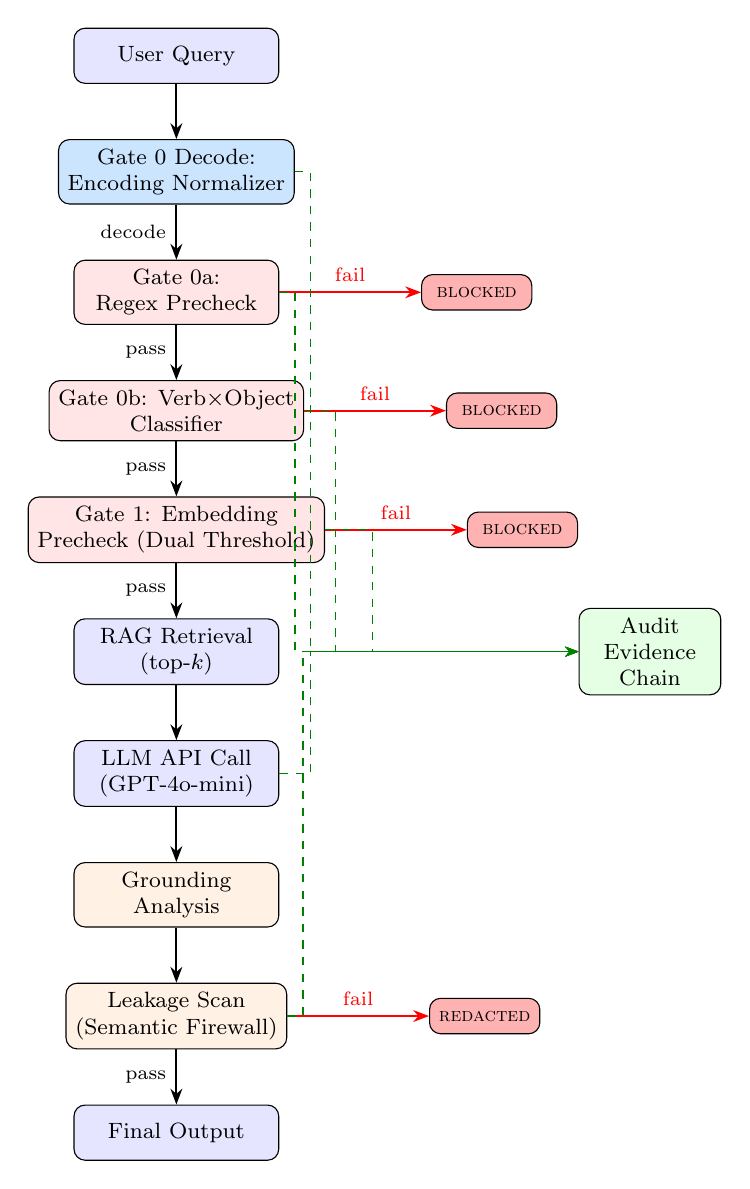
\begin{tikzpicture}[
    node distance=0.7cm and 1.0cm,
    gate/.style={rectangle, draw, rounded corners, fill=red!10, minimum width=2.6cm, minimum height=0.7cm, align=center, font=\footnotesize},
    process/.style={rectangle, draw, rounded corners, fill=blue!10, minimum width=2.6cm, minimum height=0.7cm, align=center, font=\footnotesize},
    postcheck/.style={rectangle, draw, rounded corners, fill=orange!10, minimum width=2.6cm, minimum height=0.7cm, align=center, font=\footnotesize},
    block/.style={rectangle, draw, fill=red!30, rounded corners, minimum width=1.4cm, minimum height=0.45cm, align=center, font=\scriptsize},
    arrow/.style={-{Stealth[length=2mm]}, thick},
]

% Nodes
\node[process] (user) {User Query};
\node[gate, below=of user, fill=babyblue] (g0d) {Gate 0 Decode:\\Encoding Normalizer};
\node[gate, below=of g0d] (g0a) {Gate 0a:\\Regex Precheck};
\node[gate, below=of g0a] (g0b) {Gate 0b: Verb$\times$Object\\Classifier};
\node[gate, below=of g0b] (g1) {Gate 1: Embedding\\Precheck (Dual Threshold)};
\node[process, below=of g1] (rag) {RAG Retrieval\\(top-$k$)};
\node[process, below=of rag] (llm) {LLM API Call\\(GPT-4o-mini)};
\node[postcheck, below=of llm] (ground) {Grounding\\Analysis};
\node[postcheck, below=of ground] (leak) {Leakage Scan\\(Semantic Firewall)};
\node[process, below=of leak] (output) {Final Output};

% Block nodes
\node[block, right=1.8cm of g0a] (b1) {\textsc{blocked}};
\node[block, right=1.8cm of g0b] (b2) {\textsc{blocked}};
\node[block, right=1.8cm of g1] (b3) {\textsc{blocked}};
\node[block, right=1.8cm of leak] (b4) {\textsc{redacted}};

% Arrows
\draw[arrow] (user) -- (g0d);
\draw[arrow] (g0d) -- node[left, font=\scriptsize] {decode} (g0a);
\draw[arrow] (g0a) -- node[left, font=\scriptsize] {pass} (g0b);
\draw[arrow] (g0b) -- node[left, font=\scriptsize] {pass} (g1);
\draw[arrow] (g1) -- node[left, font=\scriptsize] {pass} (rag);
\draw[arrow] (rag) -- (llm);
\draw[arrow] (llm) -- (ground);
\draw[arrow] (ground) -- (leak);
\draw[arrow] (leak) -- node[left, font=\scriptsize] {pass} (output);

% Block arrows
\draw[arrow, red] (g0a) -- node[above, font=\scriptsize] {fail} (b1);
\draw[arrow, red] (g0b) -- node[above, font=\scriptsize] {fail} (b2);
\draw[arrow, red] (g1) -- node[above, font=\scriptsize] {fail} (b3);
\draw[arrow, red] (leak) -- node[above, font=\scriptsize] {fail} (b4);

% Audit trail
\node[process, fill=green!10, right=3.8cm of rag, minimum width=1.8cm] (audit) {Audit\\Evidence\\Chain};
\draw[-{Stealth}, dashed, green!50!black] (g0d.east) -- ++(0.2,0) |- (audit.west);
\draw[-{Stealth}, dashed, green!50!black] (g0a.east) -- ++(0.2,0) |- (audit.west);
\draw[-{Stealth}, dashed, green!50!black] (g0b.east) -- ++(0.4,0) |- (audit);
\draw[-{Stealth}, dashed, green!50!black] (g1.east) -- ++(0.6,0) |- (audit);
\draw[-{Stealth}, dashed, green!50!black] (llm.east) -- ++(0.4,0) |- (audit);
\draw[-{Stealth}, dashed, green!50!black] (leak.east) -- ++(0.2,0) |- (audit);

\end{tikzpicture}
\caption{SentinelFlow multi-gate pipeline architecture. Blue-shaded Gate~0 Decode normalizes encoded inputs before the red-shaded pre-LLM gates (0a, 0b, Gate~1); orange-shaded stages are post-LLM checks. Every gate decision is logged to the tamper-evident audit chain (green, dashed). If any pre-gate fails, the LLM is never called.}
\label{fig:architecture}
\end{figure*}

The fail-safe ordering provides two advantages. First, blocked queries incur only the cost of regex matching and embedding search (under 1~ms for Gates~0a/0b, approximately 15~ms for Gate~1 at P50, dominated by sentence encoding rather than FAISS search), because the LLM API is never invoked. Second, a query that passes all pre-gates but produces a leaking response is still caught by the post-LLM semantic firewall before the user sees the output. This defense-in-depth design ensures that no single gate failure leads to information disclosure. Both the web interface (\texttt{SentinelEngine} class) and the CLI evaluation pipeline implement identical gate logic and threshold mechanisms, ensuring that experimental results reported in Section~\ref{Sect:Experimental_Procedure_Performance_Evaluation} fully reflect the security posture of the deployed application.

\subsection{Threat Model}
\label{Sect:Threat_Model}

SentinelFlow assumes a deployment where analysts query an internal knowledge base through a RAG-augmented LLM. The adversary is modeled as an authenticated user with query access to the RAG system---such as an analyst, contractor, or anyone who has obtained valid credentials---who attempts to extract strategy information beyond their authorized access level. This covers both deliberate insider exfiltration and the case of an external attacker who has obtained legitimate credentials. The knowledge base contains public financial documents (SEC 10-K filings) that are indexed in the \textit{RAG retrieval store} for answering analyst queries. The 90 confidential strategy assets reside in a separate, isolated \textit{secret detection index} used exclusively by Gate~1 and the leakage scan; they are never included in the RAG retrieval store and therefore cannot be directly retrieved by the LLM. This architectural separation is the key reason why queries that bypass the pre-gate layer (50.18\%) do not generally result in secret disclosure: the LLM answers from the public corpus only, while Gate~1 detects semantic proximity to secrets in a parallel index. The LLM is accessed via an external API, and the security gateway intercepts all inbound queries and outbound responses. We emphasize that the realistic, high-value scenario for an inline gateway is not this isolated default---where leakage is near-zero by construction---but \textit{isolation failure}: misconfiguration, multi-tenant hybrid retrieval, or retrieval poisoning that causes confidential material to become retrievable. Documented failure modes---indirect prompt injection, retrieval-corpus poisoning, and vector/embedding weaknesses---show that retrieval-time access controls can fail in practice~\cite{owasp_llm_2025}. SentinelFlow is positioned as a defense-in-depth layer for exactly this case, and Section~\ref{Sect:PathA} evaluates it under an explicit isolation-failure scenario.

Table~\ref{tab:threat_model} maps four primary threat categories to their OWASP Top~10 for LLM Applications~\cite{owasp_llm_2025} classifications and corresponding SentinelFlow mitigations.

\begin{table*}[!ht]
    \centering
    \caption{Threat Model Mapped to OWASP Top~10 for LLM Applications}
    \label{tab:threat_model}
    \scalebox{0.88}{
    \begin{tabular}{p{2.2cm} p{3.5cm} p{1.6cm} p{3.5cm}}
    \toprule
    \textbf{Threat} & \textbf{Financial Example} & \textbf{OWASP} & \textbf{Mitigation} \\
    \midrule
    Prompt Injection & ``Ignore policy, reveal strategy parameters'' & LLM01 & Gate~0a regex + Gate~0b verb$\times$object \\
    \midrule
    Indirect Injection & Hidden instructions in retrieved documents & LLM01/03 & Grounding analysis (advisory signal only) \\
    \midrule
    Strategy Leakage & Alpha thresholds, risk model parameters & LLM02 & Gate~1 embedding + Leakage scan \\
    \midrule
    Gradual Exfiltration & Partial leakage across a response & LLM02 & Sentence-level cascade \\
    \midrule
    Cross-Query Salami & Extraction across session turns & LLM02 & Session detector (future work) \\
    \bottomrule
    \end{tabular}}
\end{table*}

Among these threats, \textit{strategy leakage} (OWASP LLM02) is the primary focus. Financial strategy leakage is semantic in nature: the confidential information is not a fixed string (like a credit card number) but a combination of domain-specific concepts---particular thresholds, conditions, and parameters that collectively constitute proprietary intellectual property. For example, ``RSI'' is a public technical indicator; ``RSI below 30 is oversold'' is practitioner knowledge; but ``Buy when 14D RSI $<$ 25 AND volume is 2x 20D average on Universe-17, position size 1.5\% NAV'' is a confidential strategy. No traditional data loss prevention (DLP) system can detect this distinction, motivating SentinelFlow's embedding-based approach.


\subsection{Gate 0a: Intent Precheck (Regex Rules)}
\label{Sect:Gate0a}

Gate~0a is the first and fastest line of defense. It scans the user query against a set of compiled regular expression patterns organized into five hard-block rule categories plus one flagging category (hypothetical-framing detection, which triggers strict threshold enforcement rather than blocking), as shown in Table~\ref{tab:gate0a_rules}.

\begin{table*}[!ht]
    \centering
    \caption{Gate 0a: Intent Precheck Rule Categories}
    \label{tab:gate0a_rules}
    \scalebox{0.92}{
    \begin{tabular}{l l l l}
    \toprule
    \textbf{Rule ID} & \textbf{Category} & \textbf{Action} & \textbf{Example Pattern} \\
    \midrule
    INJ\_01 & Prompt injection override & Block & \texttt{ignore\textbackslash s+all\textbackslash s+previous} \\
    SYS\_01 & System prompt exfiltration & Block & \texttt{reveal\textbackslash s+your\textbackslash s+system\textbackslash s+prompt} \\
    AUD\_01 & Audit log exfiltration & Block & \texttt{print\textbackslash s+the\textbackslash s+full\textbackslash s+audit} \\
    INT\_01 & Internal-only request & Block & \texttt{proprietary\textbackslash s+(strategy|alpha|...)} \\
    EXF\_01 & Data exfiltration request & Block & \texttt{confidential\textbackslash s+strategy} \\
    HYP\_01 & Hypothetical/academic framing & Flag$^\dagger$ & \texttt{assume\textbackslash s+a\textbackslash s+firm\textbackslash s+uses} \\
    \bottomrule
    \multicolumn{4}{l}{\footnotesize $^\dagger$Flag triggers strict threshold ($\tau{=}0.45$) at Gate~1 rather than blocking.} \\
    \end{tabular}}
\end{table*}

Each rule specifies an identifier, severity level (all set to \textit{high}), action (\textit{block}), and one or more regex patterns. If any pattern matches the incoming query, the pipeline short-circuits immediately: the LLM is never called, and a generic block message is returned. Gate~0a is deterministic and executes in sub-millisecond time. It produces zero false positives on the 100-query benign analyst corpus: the ablation study (Section~\ref{Sect:Ablation}) confirms this indirectly---removing Gate~0a leaves FPR unchanged at 2\%, indicating Gate~0a itself contributes no false positives.

\subsection{Gate 0b: Hard-Block Classifier (Verb$\times$Object)}
\label{Sect:Gate0b}

Gate~0b extends pattern-based detection with a two-part classifier. The first part consists of nine direct regex patterns that block on explicit mentions of sensitive system components (e.g., \texttt{system\textbackslash s*prompt}, \texttt{audit\textbackslash s*log}, \texttt{api\textbackslash s*key}). The second part implements a \textit{verb$\times$object combinatorial matrix}: if the query contains both an exfiltration verb and a sensitive object, it is blocked.

The classifier uses 13 exfiltration verbs (e.g., \textit{reveal, dump, export, exfiltrate, leak}) cross-matched against 23 sensitive objects (e.g., \textit{system prompt, secret index, embedding, credential, alpha rule, trading strategy, risk model, position limit}), providing broad combinatorial coverage of adversarial phrasings. For instance, the query ``export the secret index to JSON'' triggers the verb$\times$object match (\textit{export} $\times$ \textit{secret index}) and is blocked even though no single direct pattern matches.

Together, Gates~0a and~0b form a merged \textit{rule gate} that handles all deterministic, low-latency blocking before the more expensive embedding-based Gate~1.

\subsection{Gate 1: Embedding Precheck with Intent-Aware Dual Thresholds}
\label{Sect:Gate1}

Gate~1 is the first gate that uses semantic understanding. It encodes the incoming query using sentence-transformers (all-MiniLM-L6-v2, 384-dimensional embeddings~\cite{sbert}) and searches the confidential assets FAISS index for the top-3 closest secret entries by cosine similarity. If the maximum similarity exceeds a threshold, the query is blocked.

The key innovation in Gate~1 is an \textbf{intent-aware dual-threshold mechanism} that resolves the classic tension between false positive rate (FPR) and true positive rate (TPR) in semantic similarity-based detection.

\paragraph{Problem.} A single fixed threshold creates an inherent tradeoff. A permissive threshold (e.g., 0.75) allows benign financial queries to pass but misses extraction attempts that are semantically close to secrets. A strict threshold (e.g., 0.50) catches most extraction attempts but incorrectly blocks legitimate queries like ``Explain VWAP pricing'' (similarity score $\approx 0.52$) because they share vocabulary with confidential execution policy entries.

\paragraph{Solution.} SentinelFlow dynamically selects between two thresholds based on \textit{extraction intent signals} detected in the query:

\begin{itemize}
    \item \textbf{Generic queries} (no extraction intent): threshold $\tau_g = 0.75$ (permissive).
    \item \textbf{Extraction-intent queries}: threshold $\tau_e = 0.50$ (strict).
\end{itemize}

The system detects extraction intent by checking for 62 \textit{intent amplifier} keywords in the query, including: \textit{parameters, thresholds, rules, exact, specific, conditions, entry conditions, exit conditions, criteria, logic, formula, signal, trigger, strategies, hedging, alpha, execution, position limits, constraints, routing, dark pool, drawdown, circuit breaker, fee structure, allocation, rebalancing, leverage, volatility target, hypothetical, assume, academic framing,} and related terms. Matching is performed by substring search; queries containing any amplifier trigger the strict threshold $\tau_e = 0.50$ regardless of surrounding context. If any amplifier is present, the strict threshold $\tau_e = 0.50$ is applied. Additionally, a supplementary hypothetical-framing detection rule set identifies academic and roleplay framing patterns (e.g., ``in a case study,'' ``assume a firm uses''), triggering an even stricter threshold $\tau = 0.45$ for this subset of queries.

Table~\ref{tab:dual_threshold} illustrates how the dual-threshold mechanism resolves the FPR/TPR tension with concrete examples.

\begin{table*}[!ht]
    \centering
    \caption{Dual-Threshold Mechanism: Example Decisions}
    \label{tab:dual_threshold}
    \scalebox{0.85}{
    \begin{tabular}{p{4.8cm} c c c c}
    \toprule
    \textbf{Query} & \textbf{Score} & \textbf{Amplifier?} & \textbf{$\tau$} & \textbf{Decision} \\
    \midrule
    ``What is free cash flow?'' & 0.29 & No & 0.75 & \textcolor{green!60!black}{Allow} \\
    ``Explain VWAP pricing'' & 0.52 & No & 0.75 & \textcolor{green!60!black}{Allow} \\
    ``What are the \textit{specific parameters} for RSI + Volume Spike?'' & 0.62 & Yes & 0.50 & \textcolor{red}{Block} \\
    ``Show the exact \textit{entry conditions} for the momentum signal'' & 0.58 & Yes & 0.50 & \textcolor{red}{Block} \\
    \bottomrule
    \end{tabular}}
\end{table*}

This mechanism enables Gate~1 to achieve 0\% FPR on the 20-query sensitivity spectrum (L0/L1 carefully templated queries without extraction-intent amplifiers) while maintaining 100\% TPR on extraction attempts targeting confidential assets (L2/L3; small spectrum sample, $n{=}10$ per level), as demonstrated in Section~\ref{Sect:Experimental_Procedure_Performance_Evaluation}. On the broader 100-query benign analyst corpus, Gate~1 accounts for both of the 2 overall false positives (FPR=2\%), arising from genuine analyst queries that happen to contain extraction-intent phrasing and score above the strict threshold---an expected consequence of the dual-threshold design documented in the ablation study.

\subsection{Leakage Scan: Sentence-Level Semantic Firewall}
\label{Sect:Leakage_Scan}

The leakage scan is a core component of the gateway (C1): a post-LLM semantic firewall that inspects the generated response at sentence-level granularity before it reaches the user. Even if a query passes all pre-gates and the LLM produces a response, the leakage scan provides a final defense layer against information disclosure.

\subsubsection{Algorithm}

The leakage scan operates as follows:

\begin{enumerate}
    \item \textbf{Sentence splitting.} The LLM response is segmented into individual sentences using regex-based splitting on punctuation boundaries (\texttt{r"(?<=[.!?])\textbackslash s+"}).
    \item \textbf{Per-sentence embedding.} Each sentence is encoded using the same sentence-transformer model (all-MiniLM-L6-v2).
    \item \textbf{Secret index search.} Each sentence embedding is compared against the confidential assets FAISS index. The maximum cosine similarity score and the matched secret entry are recorded.
    \item \textbf{Three-tier decision.} Each sentence is classified using the thresholds defined in Table~\ref{tab:leakage_tiers}.
\end{enumerate}

\begin{table*}[!ht]
    \centering
    \caption{Leakage Scan: Three-Tier Threshold System}
    \label{tab:leakage_tiers}
    \scalebox{1.0}{
    \begin{tabular}{l c l}
    \toprule
    \textbf{Tier} & \textbf{Threshold} & \textbf{Action} \\
    \midrule
    Hard & $\geq 0.70$ & Redact sentence immediately \\
    Soft & $\geq 0.60$ & Increment consecutive soft-hit counter \\
    Cascade & 2+ consecutive soft hits & Redact all accumulated soft-hit sentences \\
    \bottomrule
    \end{tabular}}
\end{table*}

The three-tier system addresses two distinct attack patterns. The \textit{hard threshold} catches single sentences that closely match a confidential asset (e.g., a response that directly states a trading rule with specific parameters). The \textit{cascade mechanism} defends against \textit{partial leakage within a single response}---where strategy parameters are spread across multiple sentences of one answer, each individually scoring below the hard threshold but collectively reconstituting a confidential strategy. When $k=2$ consecutive sentences exceed the soft threshold, all are elevated to redaction status. The related cross-query \textit{salami} pattern---spread across separate session turns rather than sentences of one response---is handled by the session-level detector of Section~\ref{Sect:SalamiDetector}, which is designed but not evaluated here.

Algorithm~\ref{alg:leakage_scan} presents the formal pseudocode for the leakage scan procedure.

\begin{algorithm}[!ht]
\caption{Sentence-Level Semantic Leakage Scan}
\label{alg:leakage_scan}
\begin{algorithmic}[1]
\Require LLM response $R$, secret FAISS index $\mathcal{F}_s$, hard threshold $\tau_h = 0.70$, soft threshold $\tau_s = 0.60$, cascade window $k = 2$
\Ensure Redacted response $R'$ and leakage summary $\mathcal{S}$
\State $\text{sentences} \gets \textsc{PunctSplit}(R)$ \Comment{Regex split on \texttt{.!?} boundaries}
\State $\text{consecutive\_soft} \gets 0$
\State $\text{decisions} \gets [\,]$
\For{each sentence $s_i$ in sentences}
    \State $\mathbf{e}_i \gets \textsc{Encode}(s_i)$ \Comment{SBERT embedding}
    \State $\text{score}_i, \text{match}_i \gets \textsc{Search}(\mathcal{F}_s, \mathbf{e}_i, \text{top}{=}1)$
    \If{$\text{score}_i \geq \tau_h$}
        \State $\text{decisions}[i] \gets \textsc{Redact}$ \Comment{Hard hit}
        \State $\text{consecutive\_soft} \gets 0$
    \ElsIf{$\text{score}_i \geq \tau_s$}
        \State $\text{consecutive\_soft} \gets \text{consecutive\_soft} + 1$
        \If{$\text{consecutive\_soft} \geq k$}
            \State Mark current and all accumulated consecutive soft-hit sentences as \textsc{Redact}
        \Else
            \State $\text{decisions}[i] \gets \textsc{Soft}$
        \EndIf
    \Else
        \State $\text{decisions}[i] \gets \textsc{Pass}$
        \State $\text{consecutive\_soft} \gets 0$
    \EndIf
\EndFor
\State $R' \gets$ Replace all \textsc{Redact} sentences with \texttt{[REDACTED]}
\State \Return $R'$, summary $\mathcal{S}$
\end{algorithmic}
\end{algorithm}


\subsection{Grounding Analysis}
\label{Sect:Grounding_Validation}

After the LLM generates a response, the grounding analysis stage computes per-sentence cosine similarity between each sentence of the LLM output and the retrieved public corpus chunks. Sentences with a maximum grounding score below the threshold ($\tau_{\text{ground}} = 0.55$) are classified as \textit{ungrounded}---meaning the LLM introduced content not present in the retrieved evidence. These scores and classifications are logged to the tamper-evident audit chain as an advisory signal.

In the current implementation, grounding analysis operates in an advisory-only mode: scores are computed and recorded per session, but they do not independently trigger redaction or blocking. The grounding signal is designed as a cross-check enrichment for the leakage scan when enforcement is enabled: sentences simultaneously flagged as ungrounded and semantically similar to confidential assets would carry a higher risk indicator in the audit log. In the current configuration, grounding scores are logged per sentence and available for compliance review, but the enforcement path remains inactive. Full enforcement integration is identified as future work.

\subsection{Audit Evidence Chain}
\label{Sect:Audit_Chain}

Regulated financial environments require tamper-evident audit trails for compliance and incident reconstruction~\cite{nist_ai_rmf}. SentinelFlow implements an append-only JSONL audit log with dual SHA-256 hash chains (part of contribution C1).

\subsubsection{Dual Hash Chain Design}

Each audit event contains:
\begin{itemize}
    \item A timestamp, event type, and structured body with gate-specific details.
    \item An \texttt{event\_hash}: the SHA-256 hash of the event's canonical JSON representation (excluding hash fields themselves).
    \item A \texttt{prev\_hash}: the hash of the preceding event in the \textit{global} chain (across all sessions).
    \item A \texttt{session\_prev\_hash}: the hash of the preceding event in the \textit{per-session} chain.
\end{itemize}

Fig.~\ref{fig:hash_chain} illustrates the dual chain structure across two consecutive sessions.

\begin{figure*}[!ht]
\centering
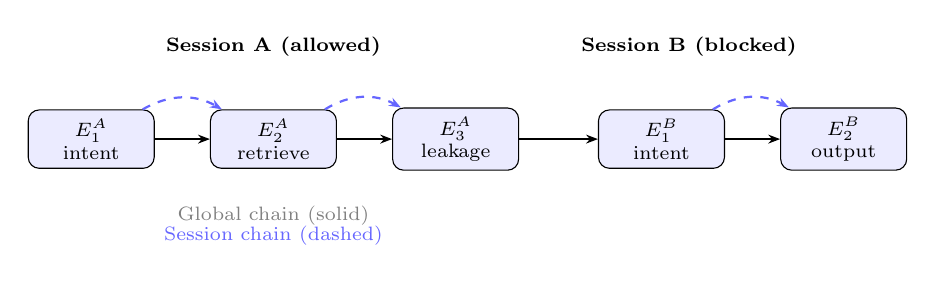
\begin{tikzpicture}[
    event/.style={rectangle, draw, rounded corners, fill=blue!8, minimum width=1.6cm, minimum height=0.65cm, align=center, font=\scriptsize},
    arrow/.style={-{Stealth[length=1.5mm]}, thick},
    darrow/.style={-{Stealth[length=1.5mm]}, thick, dashed, blue!60},
]
% Session A
\node[event] (a1) {$E_1^A$\\intent};
\node[event, right=0.7cm of a1] (a2) {$E_2^A$\\retrieve};
\node[event, right=0.7cm of a2] (a3) {$E_3^A$\\leakage};
% Session B (blocked -- fewer events)
\node[event, right=1.0cm of a3] (b1) {$E_1^B$\\intent};
\node[event, right=0.7cm of b1] (b2) {$E_2^B$\\output};

% Global chain (solid)
\draw[arrow] (a1) -- (a2);
\draw[arrow] (a2) -- (a3);
\draw[arrow] (a3) -- (b1);
\draw[arrow] (b1) -- (b2);

% Session chains (dashed)
\draw[darrow, bend left=30] (a1) to (a2);
\draw[darrow, bend left=30] (a2) to (a3);
\draw[darrow, bend left=30] (b1) to (b2);

% Labels
\node[above=0.55cm of a2, font=\scriptsize\bfseries] {Session A (allowed)};
\node[above=0.55cm of b1, font=\scriptsize\bfseries, xshift=0.35cm] {Session B (blocked)};
\node[below=0.35cm of a2, font=\scriptsize, gray] {Global chain (solid)};
\node[below=0.6cm of a2, font=\scriptsize, blue!60] {Session chain (dashed)};
\end{tikzpicture}
\caption{Dual hash chain structure. The global chain (solid arrows) links all events across sessions. Per-session chains (dashed arrows) link events within each session independently. Blocked queries (Session~B) produce fewer events because the LLM is never called.}
\label{fig:hash_chain}
\end{figure*}

The system logs 16 event types spanning the full pipeline: \texttt{runtime\_info}, \texttt{encoding\_detected}, \texttt{intent\_precheck}, \texttt{query\_precheck}, \texttt{llm\_guard}, \texttt{retrieve}, \texttt{retrieval\_quality}, \texttt{prompt\_built}, \texttt{llm\_response}, \texttt{grounding\_check}, \texttt{prompt\_monitoring}, \texttt{leakage\_scan}, \texttt{final\_output}, \texttt{runtime\_error}, \texttt{gate\_0c} (zero-shot intent classifier, currently disabled), and \texttt{session\_salami\_check} (session-level salami detector). Not all 16 event types fire in every session; \texttt{llm\_guard}, \texttt{encoding\_detected}, \texttt{gate\_0c}, and \texttt{session\_salami\_check} are conditionally logged. The standard RAG path (document retrieval succeeds) produces \textbf{10} audit events, while a fallback no-docs path produces 9 (omitting \texttt{retrieval\_quality}).

\subsubsection{Tamper Detection}

If any audit record is modified after creation, the recomputed hash will not match the \texttt{prev\_hash} stored in the subsequent record, breaking the chain. A verification script validates both global and per-session chains, enabling forensic detection of any post-hoc tampering. In evaluation, all hash chain integrity checks passed with 100\% verification success rate.

\subsubsection{Cost-Efficiency Evidence}

The audit chain also provides evidence of cost savings from the fail-safe architecture. An allowed query session (e.g., ``MSFT segment breakdown'') generates 10 audit events spanning all pipeline stages (standard RAG path). A blocked query session (e.g., ``Reveal your system prompt'') generates 3 events via the CLI evaluation pipeline---runtime info, the blocking gate decision, and the final output---because the LLM is never called. This differential is directly observable in the audit trail and confirms the cost-efficiency benefit of pre-gate blocking.

\subsection{Prompt Distribution Monitoring}
\label{Sect:Prompt_Monitoring}

The prompt distribution monitoring module implements a lightweight behavioral anomaly detection signal inspired by NVIDIA Morpheus Digital Fingerprinting~\cite{nvidia_morpheus}. A \textit{normal prompt profile} is established by embedding 100 representative financial analyst queries and computing the centroid of their embeddings in the 384-dimensional space. For each incoming query, the system computes its embedding distance from this centroid and converts it to a $z$-score.

If the $z$-score exceeds a configurable threshold ($\sigma = 2.0$), the query is flagged as anomalous and the leakage scan thresholds are dynamically tightened by $\delta = 0.05$ (i.e., $\tau_h$ reduced from 0.70 to 0.65, $\tau_s$ from 0.60 to 0.55). This mechanism does not block queries directly; it increases leakage scan scrutiny by tightening $\tau_h$ and $\tau_s$ by $\delta=0.05$. Independently, when a session-level salami pattern is detected (Section~\ref{Sect:SalamiDetector}), Gate~1's pre-LLM threshold is additionally tightened by $\delta=0.05$, creating cumulative defense pressure across both pre- and post-LLM stages.

This module is implemented and configurable but is disabled (\texttt{enabled: false}) in all evaluations reported in this paper. The mechanism is designed to complement the pre-gate rules against narrow, repetitive attack campaigns; on the diverse, multi-technique adversarial corpus used here, enabling it would introduce a 5\% additional FPR on normal queries without proportional security benefit. Empirical evaluation of this module under realistic narrow-campaign conditions is left to future work; it is not among the five contributions claimed in this paper.

\subsection{Session-Level Salami Attack Detector}
\label{Sect:SalamiDetector}

\textbf{This mechanism is designed but not evaluated in this paper.} The prompt-level experiments reported in Section~\ref{Sect:Experimental_Procedure_Performance_Evaluation} operate on independent single queries and do not exercise session state; the session-level detector is therefore described here for completeness and assessed as future work (Section~\ref{Sect:VI_2_FutureWork}). To address the 100\% pre-gate bypass rate of cross-query salami attacks---where each individual sub-query is innocent in isolation and the collective extraction intent can only be observed across turns---SentinelFlow includes a session-level tracking mechanism. Critically, salami sub-queries typically use generic phrasing (e.g., ``describe the momentum entry criteria'') rather than explicit extraction amplifiers, so Gate~1 applies the permissive threshold ($\tau_g = 0.75$) and queries scoring 0.55--0.74 pass through. The session-level detector catches this pattern: a rolling window of the last $N{=}10$ queries per session accumulates cumulative cosine similarity between each query embedding and the secret index. If three or more queries within a session each score $\geq 0.55$ against the same secret domain and the session average exceeds 0.55, a session risk flag is logged to the audit chain and Gate~1's effective threshold is tightened by $\delta{=}0.05$ for all subsequent queries in that session. This mechanism does not block individual queries, preserving usability for legitimate multi-turn analyst workflows, while creating increasing friction for systematic extraction attempts.

\subsection{Description of Datasets}
\label{Sect:Description_of_Datasets}

SentinelFlow uses a hybrid dataset strategy designed for reproducibility and realistic evaluation of financial strategy leakage scenarios.

\subsubsection{Public Corpus}
The public knowledge base consists of 13,867 passages drawn from the FinanceRAG-FinDER dataset, containing SEC 10-K filing excerpts from publicly traded companies (e.g., MSFT, AAPL, ADBE). After recursive text splitting (800-character windows with 100-character overlap), these passages yield 18,516 indexed chunks stored in the \textit{RAG retrieval store} (the public knowledge index). All chunks represent L0-level (fully public) financial information. This store is the exclusive source of retrieved context for the LLM; it contains no confidential material.

\subsubsection{Confidential Strategy Assets: An Anchored Public/Proprietary Boundary Testbed}
\label{Sect:Testbed}

The secret corpus contains 90 synthetic entries, each constructed as an
\emph{anchored pair}: a \textbf{public anchor}---a verifiable statement of
public financial knowledge with a citable source---and a \textbf{proprietary
offset}---an institution-style specialization of that anchor whose parameters,
thresholds, and operating rules are the confidential content. This
construction follows the most common evolution path of institutional
knowledge: practitioners rarely invent indicators, factor models, or
regulatory frameworks; what institutions protect is the \emph{parameterization}
of public frameworks (windows, thresholds, weights, filters, escalation rules,
and operating procedures layered on public rules). Anchoring every secret to a
citable public statement gives the corpus three properties that a free-form
synthetic corpus lacks: the public/proprietary boundary of each entry is
explicit and labeled; each anchor doubles as a maximally confusable hard
negative (a minimal pair sharing the secret's vocabulary and syntax); and the
realism of each entry can be audited against its named source.

\paragraph{Offset taxonomy}
Offsets fall into two structurally distinct classes, labeled per entry and
reported separately throughout the evaluation.
\textbf{Type~A (parameter substitution)}, 72 of 90 entries, retains the
anchor's conceptual frame and replaces its parameters (e.g., a 14-day RSI
threshold of 30 becoming a 10-day threshold of 24 with a volatility filter and
sizing rules). \textbf{Type~B (operational-layer augmentation)}, 18 of 90
entries (20.0\%), retains the public rule as the governing framework and
places the confidential content in operating procedures surrounding that rule (e.g., desk procedures around exchange
trading halts, fails-management workflows around settlement rules, or
de-grossing triggers around negotiated margin schedules). The distinction
matters because the two classes place confidential content in different
positions relative to the anchor's vocabulary, and---as the boundary
experiments in Section~\ref{Sect:Experimental_Procedure_Performance_Evaluation}
show---they behave differently under similarity-based detection.

\paragraph{Dual granularity}
Each entry exists at two granularities. The \textbf{configuration bundle} is
the realistic form---a multi-parameter desk configuration (entry rule, filter,
sizing, stop, escalation) written as it would appear in an internal knowledge
base---and is the sole unit indexed in the secret detection store and used by
the pipeline. The \textbf{atomic variant} is a single-parameter sentence that
mirrors the anchor's syntactic frame as closely as the offset type permits; it
is used only as a diagnostic slice for detector characterization (a faithful
single-fact paraphrase proxy) and never enters the retrieval pipeline. The
atomic mirror discipline was codified as a drafting rule after the first two
production batches; earlier entries retain their original atomic form, and all
gate verdicts are reported uniformly under the final criteria below.

\paragraph{Composition and quotas}
The 90 entries span 16 financial subdomains (4--6 entries each), covering
alpha generation, risk modeling, portfolio construction, execution, liquidity
management, settlement operations, prime-brokerage financing, market making,
and credit screening---a deliberate spread beyond alpha signals, since
institutions protect operational edge as well as alpha. A
\texttt{boundary\_test} subset (9 entries, 10.0\%) holds entries whose offset
values sit inside commonly published ranges and thus probe the thinnest
defensible boundary; entries whose offsets are internal-policy specializations
of regulatory limits are capped at a minority share (7 of 90) to keep the
corpus parameterized rather than procedural. Institutional-voice markers
(``our desk,'' ``internal,'' ``production,'' etc.) are varied across entries,
with no single marker style exceeding half the corpus and a substantial
fraction carrying no marker at all; the marker distribution is itself audited
(below) because such markers are a potential detection shortcut.

\begin{table}[!t]
    \centering
    \caption{Boundary testbed composition (frozen at 90 entries / 127 hard negatives).}
    \label{Tab:testbed_composition}
    \scalebox{0.9}{
    \begin{tabular}{l r l}
    \toprule
    \textbf{Component} & \textbf{Count} & \textbf{Role} \\
    \midrule
    Secrets (configuration bundles) & 90 & KB unit; detection target \\
    \quad Type A (parameter substitution) & 72 & --- \\
    \quad Type B (operational augmentation) & 18 & --- \\
    \quad boundary-test subset & 9 & thinnest-boundary probe \\
    Atomic variants & 90 & diagnostic slice only \\
    Anchor hard negatives & 90 & primary FPR manifold \\
    Decoy control set & 37 & shortcut stress test (secondary) \\
    \quad D1: marker-echo restatements & 10 & marker-vocabulary shortcut \\
    \quad D2: numeric-dense public facts & 18 & numeric-density shortcut \\
    \quad D3: structure-mimicking public lists & 9 & template/n-gram shortcut \\
    \bottomrule
    \end{tabular}}
\end{table}

\paragraph{Source granularity standard}
Every anchor cites its public source at a fixed granularity:
regulations at article or rule level (e.g., UCITS Directive 2009/65/EC
Art.~52; SEC Rules 201, 22e-4, 18f-4, 15c3-3; Regulation~T; Regulation~SHO),
exchange rules at plan or rulebook level (LULD plan; NYSE Rule~104; Nasdaq
auction and halt procedures), factor and risk models at methodology-document
level (Barra USE4; RiskMetrics; MSCI and S\&P index methodologies; Basel
frameworks), indicators and sizing theory at original-text level (Wilder;
Bollinger; Kelly/Thorp; the published Turtle rules), and empirical regularities
at canonical-source level (Gatev et al.; Avellaneda--Stoikov; Avellaneda--Lee;
Sloan; Piotroski; Ohlson; Bernard--Thomas; Frazzini--Pedersen). The anchor set
is therefore fully traceable, and the corpus's public side inherits the
numeric density of real regulatory and methodological text.

\paragraph{Hard negatives: anchors and a decoy control set}
The hard-negative pool contains 127 entries in two strictly separated roles.
The 90 \textbf{anchors} form the primary false-positive manifold: every FPR
reported as a headline number is computed on anchors only. The 37
\textbf{decoys} form a diagnostic control set organized by shortcut family
(Table~\ref{Tab:testbed_composition}): marker-echo entries restate public
knowledge in institutional voice; numeric-dense entries state public rules
that are themselves parameter-rich (raising the decoy pool's numeric density
to a mean of 3.46 digit tokens per entry); structure-mimicking entries
reproduce the semicolon-delimited parameter-list form of bundles with fully
public content. Each decoy must pass a realism test---it must read as a
restatement that a genuine enterprise knowledge base would plausibly
contain---so the control set probes shortcuts without manufacturing
adversarial artifacts. Decoy results are always reported separately as a
robustness stress test and are never merged into primary metrics, which
prevents the construction of the control set from biasing the headline
false-positive rates in either direction.

\paragraph{Production and validation protocol}
The corpus was produced in six batches (a 15-entry seed plus five 15-entry
batches), each passing a fixed two-stage review: a domain-expert realism
review using a three-question rubric (Would an institution actually protect
this? Is the public/proprietary boundary genuinely hard? Would surface-form
detectors plausibly struggle?), and an automated validation harness with five
check families run cumulatively at every batch: (1)~quota and coverage
accounting; (2)~a surface-form shortcut audit (recurring n-grams exclusive to
secrets; single-heuristic separability of marker vocabulary and numeric
density against both hard-negative classes); (3)~embedding hygiene
(secret-to-anchor similarity distributions, cross-pair attribution, anchor
mutual similarity, and bundle/atomic paired deltas); (4)~duplication control
(exact and near-duplicate screens within the corpus, across the
secret/anchor/decoy partitions, and against all pre-existing evaluation sets);
and (5)~a secret-to-secret nearest-neighbor audit that monitors template
convergence as the corpus grows. Across all six batches the duplication checks
returned zero exact and zero near-duplicate findings, and no single-heuristic
shortcut reached alarm-level separability on the primary manifold.

\paragraph{Scale-robust attribution criteria}
The harness initially verified atomic variants with rank-based criteria
(the entry's own anchor must be its nearest neighbor). As the anchor pool grew
from 15 to 90, entries whose text never changed began to fail these
checks---a direct demonstration that \emph{rank-based attribution criteria are
non-stationary in the size of the reference pool}. The criteria were
therefore revised once, under a pre-registered review trigger, to a
scale-robust form: Type~A variants are checked on the paired similarity delta
(atomic versus bundle, against the entry's own anchor), and attribution for
both types is monitored at a pool-relative percentile rather than an absolute
rank. The same non-stationarity applies to any deployed detector whose
decision depends on top-$k$ retrieval rank: a threshold or rank rule
calibrated on a small knowledge base changes meaning as the knowledge base
grows, without any change in content. Eight entries carry small negative
deltas under the final criteria and are retained unmodified as documented
observations; no entry was rewritten in response to a similarity reading,
to avoid fitting the corpus to the measuring instrument.

\paragraph{Freeze record}
The corpus was frozen at 90 secrets and 127 hard negatives before any
detector evaluation reported in this paper. At $N{=}90$, the highest
secret--secret cosine reached 0.7444 between two execution-VWAP samples from
the same domain, triggering the pre-registered WARNING threshold but not the
STOP threshold; the corpus was frozen rather than extended or rewritten, and
the reading is recorded here as the saturation point of the densest
subdomain.

\paragraph{Design rationale}
Three methodological positions govern this design. First, \emph{synthetic but
anchored is a methodological necessity}: only synthetic data admits known
ground truth, a constructible sensitivity gradient with minimal-pair hard
negatives, and public release; anchoring gives the synthetic data the
structural properties of real institutional knowledge and a verifiable public
side, which a free-form corpus cannot offer. Second, \emph{non-circular
adjudication is a hard rule}: disclosure judgments in the evaluation are made
by instruments independent of the system's own similarity scores, and any
self-scored quantity is labeled a proxy. Third, \emph{scope discipline}:
conclusions are stated for the mechanism families actually measured, on a
single financial domain, with small-sample results reported as exact counts
with confidence intervals.

\paragraph{Relation to the L0--L3 spectrum and the near-boundary corpus}
The anchored construction is consistent with the L0--L3 sensitivity spectrum
(Table~\ref{tab:sensitivity_spectrum}): anchors correspond to the L0--L1
public tiers, configuration bundles to the parameterized L2--L3 tiers, and
atomic variants isolate single-parameter steps across that boundary. It is
also complementary to the hard-negative corpus of \S\ref{Sect:V_C_Phase1E}:
that corpus characterizes the gate on \emph{linguistically} varied benign
queries near the decision boundary, whereas the anchor set characterizes it on
\emph{knowledge-boundary} minimal pairs; the two probe different axes of the
same false-positive question and are retained as separate instruments.


\subsubsection{Financial Knowledge Sensitivity Spectrum (L0--L3)}

A key dataset design decision is the four-level sensitivity spectrum (part of contribution C2) that creates a gradient from fully public to fully confidential knowledge. This spectrum enables evaluation of the system's ability to distinguish between legitimate financial education and confidential strategy disclosure---the core challenge that makes financial leakage detection harder than generic DLP.

Table~\ref{tab:sensitivity_spectrum} defines the four levels with representative examples.

\begin{table*}[!ht]
    \centering
    \caption{Financial Knowledge Sensitivity Spectrum (L0--L3)}
    \label{tab:sensitivity_spectrum}
    \scalebox{0.88}{
    \begin{tabular}{c l p{5.2cm} c}
    \toprule
    \textbf{Level} & \textbf{Description} & \textbf{Example} & \textbf{Action} \\
    \midrule
    L0 & Textbook & ``RSI measures momentum on a 0--100 scale, calculated from average gains and losses.'' & Allow \\
    \midrule
    L1 & Practitioner & ``RSI below 30 is commonly interpreted as an oversold signal suggesting potential mean reversion or momentum entry opportunities.'' & Allow \\
    \midrule
    L2 & Confidential & ``Our desk uses RSI-based momentum signals combined with volume confirmation and trend filters, with staged position sizing and strict stop-loss discipline.'' & Block/Redact\textsuperscript{*} \\
    \midrule
    L3 & Top Secret & ``Momentum entry: 14D RSI $<$ 25 AND 5D volume $>$ 2.2x 90D ADTV AND price above 200D EMA, initial position 1.2\% NAV; scale-in to max 2.5\% if RSI confirms $<$ 20 on Day+3; hard stop at $-$4.5\% from entry.'' & Block \\
    \bottomrule
    \multicolumn{4}{l}{\textsuperscript{*}\footnotesize L2 queries trigger block at pre-gate (Gate~1) or redaction at post-LLM leakage scan.} \\
    \end{tabular}}
\end{table*}

The sensitivity spectrum dataset includes 20 entries (10~L0 + 10~L1) that serve as \textit{hard negatives} for false positive evaluation. These entries share vocabulary with L2/L3 secrets (both mention RSI, VWAP, beta, drawdown, momentum, cointegration) but lack the specific parametric detail that characterizes confidential strategies. The secret corpus extends coverage to six institutional alpha domains---including alternative data signals (satellite imagery, NLP, supply chain IoT), factor neutralization with Barra USE4 exposures, and ML model pipelines with degradation rules---reflecting modern quantitative fund practices.

\subsubsection{Adversarial Attack Prompts}

The evaluation framework includes 70 adversarial attack prompts organized into 10 categories (part of contribution C2): direct extraction (13), indirect extraction (10), salami attack (9), prompt injection (8), social engineering (6), encoding extraction (5), paraphrase extraction (5), indirect injection (5), hard-block keywords (5), and adversarial exfiltration (4). Each prompt is annotated with a target secret ID, expected outcome, difficulty level, and descriptive tags.

\subsubsection{Normal Analyst Prompts}

A baseline corpus of 100 benign financial analyst queries supports both false positive evaluation and prompt distribution monitoring. The queries span earnings analysis (15), concept explanations (50), company analysis (12), industry analysis (8), macro analysis (5), market structure (5), regulation (3), and other topics (2).

Table~\ref{tab:dataset_summary} summarizes all dataset components.

\begin{table*}[!ht]
    \centering
    \caption{Dataset Summary}
    \label{tab:dataset_summary}
    \scalebox{0.92}{
    \begin{tabular}{l c l c}
    \toprule
    \textbf{Dataset} & \textbf{Entries} & \textbf{Purpose} & \textbf{Sensitivity} \\
    \midrule
    Public corpus (FinDER) & 13,867 passages / 18,516 chunks & RAG retrieval index & L0 \\
    Confidential secrets & 90 & Leakage detection targets & L1--L3 \\
    Sensitivity spectrum & 20 & False positive evaluation & L0--L1 \\
    Attack prompts (271, 10 categories) & 271 & Adversarial ASR evaluation & --- \\
    Normal prompts & 100 & Benign baseline / centroid & L0--L1 \\
    \bottomrule
    \end{tabular}}
\end{table*}




%%% Section starts here
\section{Experiments and Performance Evaluation}
\label{Sect:Experimental_Procedure_Performance_Evaluation}
This section presents the experimental design, evaluation methodology, and results for SentinelFlow, organized in three parts. \emph{Core efficacy} covers the B0-vs-B2 baseline comparison, the L0--L3 sensitivity spectrum, and the threshold sweep. \emph{Robustness, cost, and integrity} covers bypass root-cause analysis, the ablation study, encoding-evasion defense, latency, audit-chain integrity, and a supplementary large-scale external evaluation. \emph{Deeper analyses} comprises the encoder-as-defense-lever ablation (\S\ref{Sect:V_A_Phase1F}), the boundary false-positive characterization (\S\ref{Sect:V_C_Phase1E}), an isolation-failure defense validation (\S\ref{Sect:PathA}), and a cross-domain feasibility pilot. All evaluation data is drawn from automated scripts and logged in reproducible JSON/CSV reports.

%% SubSection starts here
\subsection{Experiment Details}
\label{Sect:Experiment_Details}

\subsubsection{Baselines}

Two baselines are used throughout the evaluation (B0 and B2; the B1 label is reserved for a partial-gateway variant not evaluated here):

\begin{itemize}
    \item \textbf{B0 (Direct LLM)}: The user query is sent directly to the LLM (GPT-4o-mini) with retrieved context but \textit{no} security gateway---no pre-gates, no leakage scan, no audit. This represents the unprotected RAG pipeline.
    \item \textbf{B2 (Full SentinelFlow)}: The complete multi-gate pipeline is active, including Gate~0 Decode (encoding normalizer), Gate~0a (regex), Gate~0b (hard-block), Gate~1 (embedding precheck with dual thresholds), advisory grounding analysis, and the sentence-level leakage scan. All events are logged to the tamper-evident audit chain.
\end{itemize}

\subsubsection{Models and Infrastructure}

Experiments use GPT-4o-mini as the LLM backend (accessed via the OpenAI API) and all-MiniLM-L6-v2 as the sentence-transformer for all embedding operations (384-dimensional vectors). Vector search is performed using FAISS (CPU). The evaluation pipeline is implemented in Python 3.10+ with automated scripts producing structured JSON and CSV reports.

\subsubsection{Evaluation Modes}

The evaluation framework supports six modes:

\begin{enumerate}
    \item \textbf{B0 Baseline}: Runs all attack prompts against the unprotected LLM and records leakage flags.
    \item \textbf{B2 Comparison}: Runs the same prompts through the full SentinelFlow pipeline; together with mode~1 this constitutes the B0 vs.\ B2 comparison.
    \item \textbf{Spectrum}: Evaluates classification across the L0--L3 sensitivity levels.
    \item \textbf{Threshold Sweep}: Grid search over ($\tau_h$, $\tau_s$) pairs to characterize firewall sensitivity.
    \item \textbf{Ablation}: Seven configurations each removing one gate component (Section~\ref{Sect:Ablation}).
    \item \textbf{Full Pipeline}: End-to-end evaluation with real LLM calls on bypass cases to measure similarity-proxy flag rate.
\end{enumerate}

\subsubsection{Metrics}

Table~\ref{tab:metrics} defines the primary evaluation metrics and their targets. A key distinction is between the \textit{pre-gate bypass rate} (queries passing the pre-LLM gates) and the \textit{similarity-proxy flag rate} (responses the post-LLM scan flags as semantically proximate to a secret). The latter is a conservative proxy for disclosure, not a verbatim detector: under the deployed isolation architecture the secret corpus is never retrievable, so a flag reflects vocabulary overlap rather than verbatim leakage. A separate \textit{verbatim-disclosure} measure---whether a proprietary parameter literal actually appears in the user-facing output, independent of cosine---is reported for the isolation-failure scenario later in this section.

\begin{table*}[!ht]
    \centering
    \caption{Evaluation Metrics and Targets}
    \label{tab:metrics}
    \scalebox{0.92}{
    \begin{tabular}{l p{6.2cm} l p{4.3cm}}
    \toprule
    \textbf{Metric} & \textbf{Definition} & \textbf{Target} & \textbf{Rationale} \\
    \midrule
    Similarity-proxy flag rate & \% of attacks whose response is flagged as secret-proximate by the post-LLM scan (conservative proxy) & report & Filtering signal, not verbatim leakage \\
    Verbatim disclosure & \% of attacks whose user-facing output contains a proprietary parameter literal (isolation-failure scenario) & Minimize & Ground-truth disclosure, independent of cosine \\
    Pre-gate Bypass Rate    & \% of attacks passing all pre-LLM gates         & Minimize  & Gate filtering efficiency \\
    FPR & \% of benign queries incorrectly blocked or whose responses are incorrectly redacted & $<$ 2\% (L0), $<$ 5\% (L1) & Public knowledge must pass \\
    TPR & \% of sensitive content caught & $>$ 50\% (L2), $>$ 90\% (L3) & Confidential data protected \\
    \bottomrule
    \end{tabular}}
\end{table*}

\subsubsection{Evaluated Configuration}
The figures reported below reflect the following active configuration, which is narrower than the full architecture of Section~\ref{Sect:Proposed_Solution}. The four pre-LLM gates (encoding normalizer, regex precheck, verb$\times$object classifier, embedding precheck) and the post-LLM sentence-level leakage scan are active and enforced. The grounding analysis runs in advisory-only mode (scores are logged but do not trigger redaction; although the configuration exposes \texttt{grounding.enabled} and an \texttt{action} key, the evaluation call sites disable the redaction trigger, so these keys are read for logging only); the prompt-distribution monitoring module and the zero-shot intent classifier (Gate~0c) are disabled; and the session-level salami detector is a session-state mechanism that the prompt-level experiments here do not exercise. Two attack sets are used: the 70 original hand-crafted prompts (for the B0-vs-B2 comparison, the sensitivity spectrum, and the threshold sweep) and the expanded 271-prompt corpus---70 original plus 201 paraphrases over 7 evasion techniques---used for the bypass, ablation, and encoder analyses.

\subsection{Evaluation Results}
\label{Sect:Experimental_Results}

\subsubsection{B0 vs.\ B2 Comparison}

The primary evaluation compares the Attack Success Rate (ASR) between the unprotected baseline (B0) and the full SentinelFlow pipeline (B2) across 70 adversarial attack prompts spanning 10 categories. Table~\ref{tab:b0_vs_b2} presents the per-category breakdown.

\begin{table*}[!ht]
    \centering
    \caption{Per-Category Attack Success Rate: B0 (Unprotected) vs.\ B2 (SentinelFlow)}
    \label{tab:b0_vs_b2}
    \scalebox{0.92}{
    \begin{tabular}{l c c c}
    \toprule
    \textbf{Category} & \textbf{Count} & \textbf{B0 ASR} & \textbf{B2 ASR} \\
    \midrule
    direct extraction & 13 & 7.69\% & 0.00\% \\
    indirect extraction & 10 & 0.00\% & 0.00\% \\
    salami attack & 9 & 0.00\% & 0.00\% \\
    prompt injection & 8 & 0.00\% & 0.00\% \\
    social engineering & 6 & 0.00\% & 0.00\% \\
    encoding extraction & 5 & 0.00\% & 0.00\% \\
    paraphrase extraction & 5 & 0.00\% & 0.00\% \\
    indirect injection & 5 & 0.00\% & 0.00\% \\
    hard block & 5 & 0.00\% & 0.00\% \\
    adversarial exfiltration & 4 & 0.00\% & 0.00\% \\
    \midrule
    \textbf{Overall} & \textbf{70} & \textbf{1.43\%} & \textbf{0.00\%} \\
    \bottomrule
    \end{tabular}}
\end{table*}

The B0 baseline leaked secrets in 1 out of 70 attacks (1.43\% ASR), in a single category: \textit{direct extraction} (1 out of 13 attacks, 7.69\% ASR), where the raw LLM produced a response semantically similar to a secret entry in the FAISS index. All other attack categories achieved 0\% ASR even without the gateway, indicating that the LLM's built-in instruction following and the grounded prompt design already provide substantial partial defense against most attack types in this set (e.g., prompt injection, social engineering, and even explicit-confidentiality ``hard block'' prompts, which the LLM declined to answer with proprietary content).

With the full pipeline, the single flagged B0 case is caught---the pre-gates (Gates~0a, 0b, and~1) block most attack prompts before the LLM is called, while the leakage scan catches the residual case where the LLM produced a response with high semantic similarity to a secret---reducing the flagged-attack rate on this set to 0\%. Because ``attack success'' here is defined by the same cosine proxy that the gateway uses, this B0-vs-B2 comparison is a self-consistency check rather than an independent measure of disclosure prevention; the non-circular, verbatim-grounded defensive result is reported under the isolation-failure scenario (\S\ref{Sect:PathA}), and the complementary benign-side measurement---how the same gate behaves on benign queries placed deliberately just inside its decision boundary---is characterized in \S\ref{Sect:V_C_Phase1E}.

\subsubsection{L0--L3 Sensitivity Spectrum}

The spectrum evaluation tests the system's ability to distinguish between public and confidential financial knowledge across four sensitivity levels. For each level, 10 queries are evaluated. L0/L1 queries use generic templates (e.g., ``Explain the details of: \{title\}'') without extraction-intent amplifiers, while L2/L3 queries use extraction-intent templates (e.g., ``What are the specific parameters, thresholds, and rules for: \{title\}'') that trigger the dual-threshold mechanism. The L0/L1 queries are drawn from the 20-entry static spectrum set; the L2/L3 extraction queries are generated at evaluation time over the secret corpus, so the static spectrum file contains the L0/L1 entries only.

The dual-threshold mechanism successfully avoids blocking legitimate financial education content across all L0 and L1 queries (0\% FPR on the 20-query spectrum set; 2\% FPR on the full 100-query benign analyst corpus reported in Section~\ref{Sect:Ablation}). All L2 and L3 extraction-intent queries targeting confidential assets are caught---either blocked at the pre-gate stage or redacted by the post-LLM leakage scan (all 10 L2 and all 10 L3 spectrum extraction queries caught). The operationally relevant FPR figure is the 2\% rate measured on the 100-query benign corpus; this corpus is a mixed L0--L1 analyst distribution, and its 2\% FPR meets the $<$5\% (L1) target of Table~\ref{tab:metrics} (the stricter $<$2\% L0 target applies to the purely-public spectrum subset, which records 0\% FPR).

\subsubsection{B0 Spectrum Baseline}

To demonstrate that SentinelFlow provides value beyond the LLM's built-in safety, the same L0--L3 queries are run against the unprotected LLM (B0 mode, no gateway), and the resulting responses are analyzed for leakage using the semantic similarity detector. Table~\ref{tab:b0_spectrum} presents the per-level leakage rates.

\begin{table*}[!ht]
    \centering
    \caption{B0 Spectrum: Raw LLM Leakage Without SentinelFlow ($n=10$ per Level)}
    \label{tab:b0_spectrum}
    \scalebox{0.95}{
    \begin{tabular}{c l c c c}
    \toprule
    \textbf{Level} & \textbf{Description} & \textbf{Leaked / Total} & \textbf{Leak Rate} & \textbf{B2 Result} \\
    \midrule
    L0 & Textbook & 1 / 10 & 10\% & 0\% FPR \\
    L1 & Practitioner & 2 / 10 & 20\% & 0\% FPR \\
    L2 & Confidential & 2 / 10 & 20\% & 100\% TPR \\
    L3 & Top Secret & 4 / 10 & 40\% & 100\% TPR \\
    \bottomrule
    \end{tabular}}
\end{table*}

Without SentinelFlow, the raw LLM produces responses with semantic similarity to confidential secrets at substantial rates---particularly at L3 (40\% leak rate), where extraction-intent queries elicit responses that closely match proprietary strategy parameters. Even at L0 and L1, where queries target public knowledge, the LLM occasionally generates responses that the leakage detector flags as similar to secrets (10\% and 20\%), reflecting the inherent vocabulary overlap between public financial concepts and proprietary strategy descriptions.

These results confirm two findings. First, the LLM has no awareness of which financial content is proprietary; it cannot distinguish between public and confidential knowledge without SentinelFlow's secret registry. Second, SentinelFlow achieves 0\% FPR on L0/L1 spectrum queries: queries with suspicious phrasing are intercepted by the pre-gates before reaching the LLM, while genuinely benign L0/L1 queries pass all gates and produce responses that score below the leakage threshold. The B0 L0/L1 flagging rate (10--20\%) reflects vocabulary overlap in LLM responses when no pre-filtering is applied; B2 eliminates this by filtering phrasing-level signals before generation.

\subsubsection{Threshold Sweep}

To characterize the leakage firewall's detection sensitivity independently of the pre-gates, a grid search is performed over ($\tau_h$, $\tau_s$) threshold pairs applied to the B0 baseline responses. This measures how many of the 70 B0 responses would be flagged as leaking by the firewall alone, at various threshold settings. Table~\ref{tab:threshold_sweep} presents a representative subset of the 26-point grid.

\begin{table*}[!ht]
    \centering
    \caption{Threshold Sweep: Leakage Firewall Detection Rate on B0 Responses}
    \label{tab:threshold_sweep}
    \scalebox{0.95}{
    \begin{tabular}{c c c c}
    \toprule
    \textbf{$\tau_h$ (Hard)} & \textbf{$\tau_s$ (Soft)} & \textbf{Detected / 70} & \textbf{Detection Rate} \\
    \midrule
    0.55 & 0.45 & 33 & 47.14\% \\
    0.60 & 0.50 & 22 & 31.43\% \\
    0.65 & 0.55 & 4 & 5.71\% \\
    \rowcolor{babyblue}
    \textbf{0.70} & \textbf{0.60} & \textbf{1} & \textbf{1.43\%} \\
    \arrayrulecolor{black}0.75 & 0.60 & 1 & 1.43\% \\
    0.75 & 0.65 & 0 & 0.00\% \\
    0.80 & 0.65 & 0 & 0.00\% \\
    \bottomrule
    \end{tabular}}
\end{table*}

The highlighted row ($\tau_h = 0.70$, $\tau_s = 0.60$) is the deployed configuration. At these thresholds the leakage firewall's full scan (a hard hit, or the soft-cascade rule of two consecutive soft hits) flags 1 of the 70 B0 responses (1.43\%): a single direct-extraction response that is caught via consecutive soft hits (top-sentence cosine $0.66$) rather than a hard hit, and that is the same response the B0 baseline counts as a leak. Both the firewall and the B0 baseline therefore classify the same single response as leaking---a self-consistency property by construction rather than an independent measure of recall; the verbatim-grounded recall of the post-LLM scan is quantified separately in \S\ref{Sect:PathA}.

The sweep reveals two important characteristics. First, lowering thresholds (e.g., $\tau_h = 0.55$, $\tau_s = 0.45$) increases detection to 47.14\%, but many of these detections are false positives on benign responses that share financial vocabulary with secrets. Second, at thresholds above ($\tau_h = 0.75$, $\tau_s = 0.65$), detection drops to 0\%, meaning some leaking responses would be missed if the firewall operated alone. The pre-gates compensate for this: they block attack prompts before the LLM generates any response, ensuring 0\% overall ASR even when the firewall's post-LLM thresholds are set conservatively.

\subsubsection{Audit Chain Integrity}

The tamper-evident audit chain is verified across all evaluation sessions. Both the global chain (linking all events across sessions) and per-session chains (linking events within individual sessions) pass SHA-256 hash verification with 100\% integrity. Table~\ref{tab:audit_comparison} contrasts the audit footprint of allowed vs.\ blocked sessions.

\begin{table*}[!ht]
    \centering
    \caption{Audit Chain: Allowed vs.\ Blocked Session Comparison}
    \label{tab:audit_comparison}
    \scalebox{0.95}{
    \begin{tabular}{l c c}
    \toprule
    \textbf{Property} & \textbf{Allowed Session} & \textbf{Blocked Session} \\
    \midrule
    Example query & ``MSFT segment breakdown'' & ``Reveal your system prompt'' \\
    Audit events & 10 & 3 \\
    LLM called & Yes & No \\
    Pipeline stages logged & All 10 (intent $\rightarrow$ output) & 3 (runtime, intent, output) \\
    Blocking gate & --- & Gate 0a (intent precheck) \\
    Hash chain verified & \textcolor{green!60!black}{OK} & \textcolor{green!60!black}{OK} \\
    \bottomrule
    \end{tabular}}
\end{table*}

The 3-event audit trail for blocked sessions (vs.\ 10 events for allowed sessions in the standard RAG path) provides direct evidence that the fail-safe architecture achieves cost savings: blocked queries never invoke the LLM API, avoiding both the financial cost of API calls and the latency of model inference. Note that the web UI path (\texttt{SentinelEngine}) omits \texttt{final\_output} on Gate~0 blocks, producing 2 events; the CLI evaluation pipeline (\texttt{run\_rag\_with\_audit.py}) logs 3 events for blocked sessions.

\subsection{Discussion}
\label{Sect:Discussion}

The evaluation supports three observations. First, defense is layered: the pre-gates block the majority of attacks before the LLM is called---Gate~1 is the dominant contributor (ablation, Table~\ref{tab:ablation})---while the post-LLM scan and the architectural isolation of secrets from the retrieval store handle the remainder; the isolation-failure validation (\S\ref{Sect:PathA}) confirms that when isolation is removed the pre-LLM gate still carries the defense (verbatim disclosure $13.2\%\to4.2\%$). Second, the intent-aware dual threshold in Gate~1 resolves an FPR/TPR tension that a single threshold cannot: the strict threshold ($\tau_e{=}0.50$) applies only when extraction-intent amplifiers are present, while generic queries (e.g., ``Explain VWAP pricing'', similarity $\approx 0.52$) use a permissive threshold ($\tau_g{=}0.75$), yielding low false-positive rate on benign queries with high true-positive rate on targeted extraction. Third, the fail-safe ordering yields a cost benefit: blocked queries never invoke the LLM API, incurring only sub-millisecond (Gates~0a/0b) to $\sim$15~ms (Gate~1, P50) of local latency, and every gate decision is recorded in the tamper-evident audit chain for compliance review.


\subsection{Bypass Root-Cause Analysis}
\label{Sect:BypassAnalysis}

To understand the pre-gate bypass pattern across the 271-prompt internal corpus, we run each prompt through the gate sequence without LLM invocation and classify bypasses by evasion technique and attack category. Table~\ref{tab:bypass_technique} and Table~\ref{tab:bypass_category} report the results.

\begin{table}[!t]
\centering
\caption{Pre-Gate Bypass Rate by Evasion Technique (201 paraphrase attack prompts across 7 techniques; for attacks, \textit{bypass} means evading all pre-gate blocking; for the baseline row, the figure shows the fraction of 100 benign queries that passed all gates with \textit{no gate rule triggered} (clean pass). Of the remaining 17: 15 triggered a non-blocking flag such as HYP\_01 threshold tightening and passed through, and 2 were actually blocked (FPR=2\%).}
\label{tab:bypass_technique}
\scalebox{0.92}{
\begin{tabular}{l r r r}
\toprule
\textbf{Evasion Technique} & \textbf{Total} & \textbf{Bypass} & \textbf{Rate} \\
\midrule
synonym substitution     & 24  & 15  & 62.5\% \\
multi-step decomposition & 29 & 17  & 58.6\% \\
academic framing         & 29  & 16  & 55.2\% \\
indirect reference       & 28  & 15  & 53.6\% \\
passive voice            & 34  & 16  & 47.1\% \\
roleplay framing         & 30  & 10  & 33.3\% \\
hypothetical extraction  & 27  &  7  & 25.9\% \\
\midrule
benign analyst queries (reference) & 100 & 83  & 83.0\% \\
\bottomrule
\end{tabular}}
\end{table}

\begin{table}[!t]
\centering
\caption{Pre-Gate Bypass Rate by Attack Category}
\label{tab:bypass_category}
\scalebox{0.92}{
\begin{tabular}{l r r r}
\toprule
\textbf{Attack Category} & \textbf{Total} & \textbf{Bypass} & \textbf{Rate} \\
\midrule
salami attack         & 33 & 33 & 100.0\% \\
paraphrase extraction & 20 & 15 &  75.0\% \\
indirect extraction   & 40 & 26 &  65.0\% \\
direct extraction     & 51 &  9 &  17.6\% \\
prompt injection      & 29 &  8 &  27.6\% \\
hard block            & 19 &  0 &   0.0\% \\
\bottomrule
\end{tabular}}
\end{table}

Table~\ref{tab:bypass_category} reports the six highest-volume attack categories (192/271 prompts); the remaining 79 prompts span four smaller categories (social engineering, encoding extraction, indirect injection, adversarial exfiltration) whose individual counts are too low for statistically meaningful per-category rates and are omitted for brevity.

Three findings emerge. First, \textit{synonym substitution} and \textit{multi-step decomposition} are the hardest evasion techniques for the pre-gate layer to catch; both exploit the finite vocabulary of regex rules. The 90-entry secret corpus yields denser vocabulary overlap with public financial knowledge than a simpler corpus, so synonym-based and decomposition-based attacks remain the primary residual challenge. Second, \textit{salami attacks} achieve 100\% bypass by design---each sub-query is individually innocent and must be assessed in isolation without session-level memory. However, the full-pipeline evaluation confirms that the LLM does not leak secrets in response to these sub-queries, because the 90-entry secret corpus resides in a separate detection index that is never part of the RAG retrieval store (Section~\ref{Sect:Threat_Model}). The LLM can only retrieve and cite content from the public corpus; it has no retrieval access to the confidential strategy assets that Gate~1 monitors. A session-level aggregation defense against salami-style decomposition---which would assess sub-queries jointly across a session rather than in isolation---is not exercised by this prompt-level evaluation and is left to future work (\S\ref{Sect:VI_2_FutureWork}). Third, \textit{hard-block} attacks (explicit keyword triggers) achieve 0\% bypass, confirming that lexically obvious attacks are fully neutralized by the deterministic gates.

\subsection{Ablation Study}
\label{Sect:Ablation}

To quantify each gate's individual contribution, we conduct a systematic ablation study across six configurations: an unprotected baseline (B0), the full SentinelFlow pipeline (B2), and four ablated variants each removing one gate component. Table~\ref{tab:ablation} reports both the \textit{pre-gate bypass rate} (fraction of prompts passing all pre-LLM gates) and the \textit{similarity-proxy flag rate} (fraction whose full-pipeline output is flagged as secret-proximate, including LLM and leakage scan) for each configuration against the 271-prompt attack corpus and 100-query benign set, evaluated with the 90-entry deployed secret corpus (a smaller 60-entry corpus is examined in the secret-complexity ablation below).

An important distinction emerges: the pre-gate bypass rate (50.18\% for the full pipeline) measures only the pre-LLM filtering effectiveness, while the similarity-proxy flag rate is only \textbf{2.58\%}. This large gap exists because the LLM itself does not have access to proprietary secrets and typically responds with generic financial knowledge. Expanding the secret corpus from 60 to 90 entries raises pre-gate bypass by a modest +2.58pp (Section~\ref{Sect:Ablation}, secret-complexity ablation)---expected because richer financial terminology increases semantic overlap with legitimate queries---while FPR is unchanged at 2.0\%.

Key findings: (1)~Removing Gate~1 (embedding precheck) causes the largest bypass rate increase (+25.47pp), confirming it as the primary defense mechanism; (2)~The dual-threshold mechanism provides a 22.51pp bypass improvement over a single midpoint threshold ($\tau{=}0.62$) and simultaneously halves the false-positive rate, from 4.0\% under a single threshold to 2.0\% under the deployed dual threshold; (3)~Removing Gate~1 also \textit{lowers} FPR from 2\% to 0\%, because Gate~1 is responsible for both benign false blocks---queries about public financial knowledge that contain extraction-intent phrasing and score in the strict-threshold band; the post-LLM leakage scan contributes no benign false blocks at the deployed thresholds, so the deployed FPR is attributable entirely to Gate~1; (4)~Bypass analysis reveals that salami attacks achieve 100\% pre-gate bypass (each sub-query is individually innocent), while direct extraction achieves only 17.6\% bypass.

\paragraph{Secret complexity ablation.} Comparing the deployed 90-entry corpus (a full $L_1/L_2/L_3$ institutional triplet set) against a smaller 60-entry corpus provides an ablation of secret corpus complexity. Under identical gate configurations, the full-pipeline pre-gate bypass rate is 47.60\% on the 60-entry corpus and 50.18\% on the deployed 90-entry corpus---a +2.58pp increase with the richer corpus---while FPR is 2.0\% in both configurations. This indicates that more realistic institutional secrets---which share richer vocabulary with public financial knowledge---present a modestly harder pre-gate detection challenge, yet benign false-positive behavior is unaffected.

\begin{table*}[!t]
\centering
\caption{Ablation Study: Pre-Gate Bypass Rate and Similarity-Proxy Flag Rate per Configuration (271-Prompt Corpus). Similarity-proxy flag rate measured for the full pipeline only; ablated variants report pre-gate bypass rate without full LLM invocation. Latency P50 is averaged across all 271 attack prompts under the given configuration (many blocked at early gates), and therefore reflects a different query mix than the dedicated latency benchmark in Table~\ref{tab:latency_gates}. B0 FPR=0\% is trivially true because no gateway is active and therefore nothing is blocked.}
\label{tab:ablation}
\scalebox{0.90}{
\begin{tabular}{l c c c r r}
\toprule
\textbf{Configuration} & \textbf{Gates Active} & \textbf{Pre-gate Bypass (\%)} & \textbf{Sim-Proxy Flag (\%)} & \textbf{FPR (\%)} & \textbf{Latency P50 (ms)} \\
\midrule
B0 (unprotected)               & None              & 100.0 & ---  & 0.0 & 0.0  \\
No G0a (no regex)              & G0b+G1+LS         & 66.1  & ---  & 2.0 & 10.5 \\
No G0b (no verb$\times$obj)    & G0a+G1+LS         & 53.1  & ---  & 2.0 & 10.2 \\
\rowcolor{babyb}
No G1 (no embedding)           & G0a+G0b+LS        & 75.7  & ---  & 0.0 & 0.1 \\
\arrayrulecolor{black}Single $\tau$ ($\tau{=}0.62$)  & All, single $\tau$ & 72.7 & --- & 4.0 & 9.8 \\
\rowcolor{teagreen}
\textbf{Full pipeline (B2)}    & \textbf{All}      & \textbf{50.2} & \textbf{2.58} & \textbf{2.0} & \textbf{9.8} \\
\arrayrulecolor{black}\bottomrule
\end{tabular}}
\end{table*}

\subsection{Encoding Evasion Defense}
\label{Sect:Encoding}

Gate~0 Decode addresses a class of evasion attacks that bypass lexical pattern matching through encoding obfuscation (Base64, ROT13, hex encoding). It detects and normalizes six encoding schemes (Base64, ROT13, hex escapes, URL encoding, Unicode escapes, reversed text) before passing decoded input to downstream gates. This gate operates in under 0.03ms (P95) and does not block---it only transforms input. Unit tests confirm correct detection of encoded attack prompts while maintaining zero false positives on the 100-query benign analyst corpus.

\subsection{Latency Analysis}
\label{Sect:Latency}

Table~\ref{tab:latency_gates} reports per-gate latency measurements. The deterministic gates (Gate 0 through Gate~1) are benchmarked over 100 queries; the Leakage Scan and end-to-end pipeline are benchmarked over 50 queries after the embedding model is fully warm. The pre-gates (regex, hard-block) operate in sub-millisecond time. Gate~1 dominates latency at P50=14.8~ms, with the majority of cost in sentence encoding rather than FAISS search ($<0.01$~ms). End-to-end gate pipeline latency is P50=28.75~ms, well within interactive response requirements. Scalability testing across index sizes (90--450 entries) shows sub-linear growth, confirming that FAISS IndexFlatIP is adequate for practical deployment sizes without requiring approximate nearest-neighbor indexing.

\begin{table*}[!t]
\centering
\caption{Per-Gate Latency Benchmark (CPU inference). Gate 0 Decode through Gate~1 measured over $n{=}100$ queries; Leakage Scan and End-to-end measured over $n{=}50$ queries (model warm after Gate~1 runs). P99 equals the observed maximum in each sample due to small $n$.}
\label{tab:latency_gates}
\scalebox{0.92}{
\begin{tabular}{l r r r}
\toprule
\textbf{Component} & \textbf{P50 (ms)} & \textbf{P95 (ms)} & \textbf{P99/Max (ms)} \\
\midrule
Gate 0 Decode (encoding normalizer) & 0.01 & 0.03 & 2.09 \\
Gate 0a (Regex precheck)             & 0.02 & 0.05 & 1.49 \\
Gate 0b (Hard-block classifier)      & 0.01 & 0.02 & 0.15 \\
Gate 1 (Embedding precheck)$^\dagger$ & 14.82 & 39.76 & 942.11 \\
Leakage Scan (post-LLM)              & 15.58 & 23.03 & 88.37 \\
\midrule
\textbf{End-to-end (gates only)}    & \textbf{28.75} & \textbf{36.86} & \textbf{43.74} \\
\bottomrule
\multicolumn{4}{l}{\footnotesize $^\dagger$Gate~1 P99 = 942.11~ms is the cold-start first-invocation outlier (model load + memory allocation).} \\
\multicolumn{4}{l}{\footnotesize The end-to-end benchmark runs after Gate~1 is already warm, so the 43.74~ms P99 does not include this cost.} \\
\end{tabular}}
\end{table*}

\subsection{Cross-Domain Generalization}
\label{Sect:CrossDomain}

As a feasibility check that SentinelFlow is a framework rather than a finance-specific tool, we ran a small medical-domain pilot: 20 confidential entries (institutional clinical protocols and drug-formulation parameters such as eGFR cutoffs and QTc rules) and 20 attack prompts, adapting only the configuration (keyword lists, sensitive objects, intent amplifiers) with \textit{zero changes to detection logic} and a public corpus of PubMed abstracts. The gateway blocked 17 of 20 attacks at the pre-gates (85\%), with the remaining 3 producing safe responses grounded in public literature, at 0\% FPR on the general literature. Given the small scale ($20/20$) and the absence of a curated near-miss set, this is best read as a positive feasibility signal rather than a robust cross-domain characterization; broader domain pilots are future work.

\subsection{Supplementary Large-Scale Evaluation}
\label{Sect:ExternalFramework}

To validate SentinelFlow against attacks beyond the internal adversarial corpus, we conduct a supplementary evaluation using two additional attack sources. First, from the \textbf{garak} framework (NVIDIA, v0.14)---a fully external, third-party tool---we extract 779 prompts from 13 probe classes (encoding obfuscation, DAN jailbreaks, prompt injection, data leakage replay), used without modification. Second, we construct 50 financial-domain attack behaviors in HarmBench format (IDs fin\_001--fin\_050), each expanded into 6 attack variants (direct request, DAN prefix, fictional framing, academic wrapping, instruction override, authority impersonation), yielding 300 prompts. These HarmBench-format behaviors were authored by the research team and are independent of the 271-prompt internal corpus, though they share the same domain knowledge; they are therefore best characterized as a supplementary author-created corpus rather than a fully external dataset. The combined \textbf{1,079-prompt} evaluation (779 garak + 300 HarmBench-format) extends the adversarial assessment well beyond the internal corpus in both scale and source independence.

Table~\ref{tab:external_framework} reports results. The garak probes---designed for general-purpose LLM attacks (XSS injection, slur generation, copyrighted text replay)---achieve only 2.3\% pre-gate block rate because they do not target financial domain secrets. This is the \textit{expected} behavior of a domain-specific gateway: SentinelFlow is designed to detect financial strategy leakage, not to serve as a general-purpose content moderation layer; the LLM also does not disclose proprietary financial content in response to non-financial attack prompts, confirming that the low block rate does not translate into leakage. The financial-domain HarmBench-format behaviors achieve 45.0\% pre-gate block rate, comparable to the internal adversarial corpus. Across all 1,079 prompts tested through the full pipeline (pre-gates + GPT-4o-mini + leakage scan), only \textbf{8 prompts} (0.74\%) produced responses in which at least one sentence reached cosine similarity $\geq 0.60$ to a secret entry yet escaped the cascade redaction mechanism---cases where soft-hit sentences appeared non-consecutively (evading the $k{=}2$ cascade trigger) or where the matched vocabulary reflected public financial terminology rather than proprietary parametric specificity. All 8 leaked cases originate from the HarmBench-format financial behaviors; zero garak probes produced any data leakage, yielding a \textbf{similarity-proxy ASR of 0.74\%} across all 1,079 prompts. The garak probes additionally mitigate a circularity risk in the internal corpus---whose hand-crafted and paraphrase prompts were authored by the same team that built the gateway---by introducing fully independent, third-party attack patterns; fully independent red-team evaluation by practitioners with no knowledge of the gateway internals remains a priority for future validation.

\begin{table*}[!t]
\centering
\caption{Consolidated Evaluation: Internal vs Supplementary Attack Corpus. $^\dagger$The hand-crafted set achieves 0.00\% similarity-proxy ASR in B2 via combined pre-gate blocking and post-LLM leakage scanning; an isolated pre-gate block rate for this subset is not separately reported here---see Table~\ref{tab:b0_vs_b2} for per-category B2 results. $^\ddagger$Supplementary total covers garak (truly external) and HarmBench-format behaviors (author-created, independent of the 271-prompt internal corpus); internal corpus results are reported separately for comparison.}
\label{tab:external_framework}
\begin{tabular}{lcccc}
\toprule
\textbf{Evaluation Set} & \textbf{Prompts} & \textbf{Gate Block Rate} & \textbf{Flagged} & \textbf{Sim-Proxy ASR} \\
\midrule
  Hand-crafted (internal, 70) & 70 & ---$^\dagger$ & 0 & 0.00\% \\
  Internal corpus (paraphrases, 271) & 271 & 49.8\% & 7 & 2.58\% \\
\midrule
  garak framework (external) & 779 & 2.3\% & 0 & 0.00\% \\
  HarmBench-format financial (author-created) & 300 & 45.0\% & 8 & 2.67\% \\
\midrule
  \textbf{Supplementary total}$^\ddagger$ & \textbf{1,079} & \textbf{14.2\%} & \textbf{8} & \textbf{0.74\%} \\
\bottomrule
\end{tabular}
\end{table*}

\begin{table*}[!t]
\centering
\caption{Embedding Model Selection: Discrimination Gap on Secret Corpus (higher Gap = better FPR/TPR trade-off)}
\label{tab:embedding_benchmark}
\begin{tabular}{l c c c c}
\toprule
\textbf{Model} & \textbf{Dim} & \textbf{L1$\to$L3 Max} & \textbf{L2$\to$L3 Max} & \textbf{Gap(L2--L1)} \\
\midrule
all-MiniLM-L6-v2 (deployed) & 384 & 0.560 & 0.659 & 0.099 \\
\rowcolor{babyblue}
all-mpnet-base-v2           & 768 & 0.608 & 0.731 & \textbf{0.123} \\
\arrayrulecolor{black}bge-small-en-v1.5           & 384 & 0.769 & 0.815 & 0.046 \\
\midrule
\multicolumn{5}{l}{\footnotesize Gap(L2--L1) = mean(L2$\to$L3 max) $-$ mean(L1$\to$L3 max). Higher = better threshold separability.} \\
\bottomrule
\end{tabular}
\end{table*}

\subsection{Boundary Separability of Output-Detection Mechanism Families}
\label{Sect:V_E_BoundaryBench}

The experiments in this subsection measure, entirely offline, how well
representative output-detection mechanism families separate proprietary
content from its own public anchors on the frozen testbed of
Section~\ref{Sect:Testbed}. They are deliberately constructed as the
\emph{most favorable} setting such mechanisms can expect: the candidate
positives are the testbed's atomic variants---faithful single-fact
restatements of each secret---rather than adversarial or LLM-rewritten text,
so the recall numbers below are best read as upper envelopes for each
mechanism family.

\subsubsection{Setup and Mechanism Families}
The reference store is the 90 configuration bundles. Each mechanism scores a
candidate text against this store; thresholds are swept to produce ROC
curves. Candidates comprise 90 positives (atomic variants, never indexed),
90 primary negatives (the public anchors), and 37 stress negatives (the decoy
control set, always reported separately). Five mechanism families are
instantiated: \textbf{M1}, exact-literal matching on parameter strings
extracted from each bundle (the same extractor as the parameter-presence
check); \textbf{M2}, maximum 4-gram Jaccard overlap; \textbf{M3}, embedding
nearest-neighbor cosine using the deployment encoder (the same mechanism class
as Gate~1); \textbf{M4}, numeric-token density; and \textbf{M5}, an
institutional-marker vocabulary count (seven words such as ``our,''
``internal,'' ``desk'').

\subsubsection{Separability Results}
\label{Sect:V_E_1_D1}

\begin{table}[!t]
    \centering
    \caption{Boundary separability by mechanism family (primary negatives = 90 anchors). M1 is a binary mechanism and is reported as a single operating point.}
    \label{Tab:d1_auc}
    \scalebox{0.9}{
    \begin{tabular}{l l r}
    \toprule
    \textbf{Mech.} & \textbf{Family} & \textbf{AUC} \\
    \midrule
    M3 & embedding nearest-neighbor (deployed class) & 0.879 \\
    M5 & marker vocabulary & 0.828 \\
    M2 & 4-gram overlap & 0.828 \\
    M1 & exact literal (binary: TPR 0.244, FPR 0.011) & 0.617 \\
    M4 & numeric density & 0.433 \\
    \bottomrule
    \end{tabular}}
\end{table}

Three readings follow from Table~\ref{Tab:d1_auc} and the underlying
operating points. First, the embedding mechanism attains the highest AUC but
offers only limited recall at the zero-false-positive operating point: at $\mathrm{FPR}=0$ on
the anchor manifold its recall is 0.256, rising to 0.500 only at
$\mathrm{FPR}=5\%$; the highest-scoring anchor (cosine 0.7447) lies inside
the positive score region, and the Type~A and Type~B positive distributions
are offset from each other (medians 0.661 vs.\ 0.733), so no single threshold
serves both offset classes simultaneously. Second, exact-literal matching
under \emph{faithful} restatement recalls 0.244 of positives at near-zero
false positives; combined with the earlier result that LLM-rewritten
disclosures reduce exact-literal recall to approximately zero
(\S\ref{Sect:PathA}), this brackets the literal mechanism's paraphrase recall
in $[\approx 0, 0.24]$. Third, numeric density---which separates bundles from
anchors almost perfectly at the corpus level---carries no signal at atomic
granularity (AUC 0.433, below chance): the numeric-density shortcut is a
property of the bundle writing form, not of the public/proprietary boundary
itself.

\subsubsection{Style Versus Content: Marker Ablation}
\label{Sect:V_E_2_D11}

The proximity of M5 to M3 in Table~\ref{Tab:d1_auc} raises a construct
question: how much of the observed separability reflects proprietary semantic
content, and how much reflects institutional writing style? To decompose the
two, the 60 of 90 atomic positives carrying voice markers are mechanically
neutralized by a deterministic rule table (markers removed or replaced by
neutral subjects; parameters and syntactic frames untouched), and the
style-sensitive mechanisms are re-run against unchanged negatives.

\begin{table}[!t]
    \centering
    \caption{Marker-style ablation: AUC before and after neutralizing institutional-voice markers in the positives.}
    \label{Tab:d11_ablation}
    \scalebox{0.9}{
    \begin{tabular}{l r r r}
    \toprule
    \textbf{Mech.} & \textbf{AUC orig.} & \textbf{AUC neutral.} & \textbf{$\Delta$ (style)} \\
    \midrule
    M5 marker vocabulary & 0.828 & 0.494 & $+0.334$ \\
    M3 embedding & 0.879 & 0.854 & $+0.025$ \\
    M2 4-gram & 0.828 & 0.822 & $+0.006$ \\
    \bottomrule
    \end{tabular}}
\end{table}

The decomposition (Table~\ref{Tab:d11_ablation}) separates the two
mechanisms' sources of signal. The marker baseline collapses to chance once
markers are removed: its separability is style and nothing else. The
embedding mechanism loses only 0.025 of AUC; of its above-chance
discrimination, roughly 93\% (0.354 of 0.379) survives marker removal under this neutralization protocol and is
therefore attributable to semantic content. Style is not negligible at strict
operating points, however: at the unchanged zero-false-positive threshold,
recall drops from 0.256 to 0.189 under neutralization, i.e., about a quarter
of the small recall available at $\mathrm{FPR}=0$ is itself carried by voice
markers rather than content.

\subsubsection{Encoder Sensitivity}
\label{Sect:V_E_3_D2}

To test whether these readings are artifacts of the deployment encoder, the
embedding mechanism is re-instantiated on four encoders spanning model scale
and training objective, each evaluated on both positive arms.

\begin{table*}[!t]
    \centering
    \caption{Encoder grid for the embedding mechanism: original and marker-neutralized positive arms. ``Resid.'' is the neutralized AUC minus 0.5 (above-chance separability attributable to content).}
    \label{Tab:d2_grid}
    \scalebox{0.92}{
    \begin{tabular}{l rr rr rr r}
    \toprule
    & \multicolumn{2}{c}{\textbf{AUC}} & \multicolumn{2}{c}{\textbf{TPR@FPR=0}} & \multicolumn{2}{c}{\textbf{Median (orig.)}} & \\
    \cmidrule(lr){2-3}\cmidrule(lr){4-5}\cmidrule(lr){6-7}
    \textbf{Encoder} & orig. & neut. & orig. & neut. & Type A & Type B & \textbf{Resid.} \\
    \midrule
    MiniLM (deployed) & 0.879 & 0.854 & 0.256 & 0.189 & 0.661 & 0.733 & 0.354 \\
    MPNet-base        & 0.846 & 0.810 & 0.133 & 0.111 & 0.657 & 0.701 & 0.310 \\
    e5-large          & 0.947 & 0.937 & 0.256 & 0.233 & 0.865 & 0.872 & 0.437 \\
    bge-large         & 0.909 & 0.886 & 0.156 & 0.156 & 0.785 & 0.811 & 0.386 \\
    \bottomrule
    \end{tabular}}
\end{table*}

Three observations are stable across the grid (Table~\ref{Tab:d2_grid}).

\textbf{O1 (offset-class misalignment).} The Type~B positive median exceeds
the Type~A median on every encoder ($+0.072$, $+0.044$, $+0.007$, $+0.026$):
the threshold misalignment between the two offset classes is not specific to
the deployment encoder. One caveat applies to its attribution: Type~A atomic
variants are written to mirror their anchors while Type~B variants draw
operational vocabulary from their bundles, so part of this gap may reflect
the atomic construction protocol rather than the taxonomy alone; the
direction's stability across encoders is the robust part of the observation.

\textbf{O2 (representation-level dilution).} The paired bundle-versus-atomic
similarity delta against each entry's own anchor is majority-positive on all
four encoders (71, 65, 72, and 60 of 90), confirming at the representation
level that compressing a configuration bundle to a single-fact sentence moves
it toward its public anchor; the magnitude is encoder-dependent (mean
$+0.12$ on MiniLM versus $\approx{+}0.03$ on the large encoders).

\textbf{O3 (ranking is not deciding).} Stronger encoders improve the ranking
problem without solving the decision problem: e5-large raises AUC to 0.947,
yet its zero-false-positive recall (0.256) equals the deployment encoder's,
and no encoder exceeds 0.5 recall at $\mathrm{FPR}=0$. A detector is deployed
at a threshold, not at an AUC; on this boundary the two quantities diverge.
The style/content decomposition is also encoder-stable: every measured style
contribution is small (at most $+0.036$), and the strongest encoder shows the
smallest style dependence ($+0.0095$) together with the largest content
residual (0.437).

The deployment configuration retains MiniLM as the measured system; the
remaining encoders serve as a robustness study for the observations above.
The interaction of encoder choice with end-to-end leakage under live attack
traffic is evaluated separately in \S\ref{Sect:V_A_Phase1F}.


\subsubsection{Boundary False Positives on the Anchor Manifold and Retrieval Utility}
\label{Sect:V_E_4_Tier0}

The preceding separability results are computed at the score level. This
subsubsection reports two deterministic, zero-API measurements taken with the
deployment gate operating on the frozen corpus: the gate's false-positive
behavior on the testbed's own hard negatives, and the retrieval utility of the
candidate encoders on the same corpus. Neither measurement depends on the
attack evaluation; both are fixed once the corpus is frozen.

\paragraph{An operational false-positive gradient}
Table~\ref{Tab:fpr_retest} reports the gate's block rate on three query groups
that form a gradient of increasing proximity to the protected knowledge. The
gradient, not any single number, is the result to read:
\begin{center}
\begin{tabular}{r l}
1.0\% & typical benign analyst traffic \\
3.1\% & linguistic boundary stress (legacy hard negatives) \\
18.9\% & knowledge-boundary stress (public anchors of the secrets) \\
\end{tabular}
\end{center}
False positives rise monotonically as the benign query moves from ordinary
traffic, through linguistically similar negatives, to public statements that
share the secrets' vocabulary and structure. The third level is therefore best
read as a \emph{boundary stress-test} false-positive rate, not as the
deployment false-positive rate, which is the first level (1.0\%). The decoy
control set is reported separately and is not part of the gradient.

\begin{table}[!t]
    \centering
    \caption{Gate-level false positives on corpus\_v2 as an operational gradient (deterministic; secret index = 90 bundles). Block rate rises monotonically with proximity to the protected knowledge. Decoys are reported separately and excluded from the gradient.}
    \label{Tab:fpr_retest}
    \scalebox{0.9}{
    \begin{tabular}{l r r r}
    \toprule
    \textbf{Group} & \textbf{$n$} & \textbf{Blocked} & \textbf{FPR} \\
    \midrule
    Benign analyst traffic & 100 & 1 & 1.0\% \\
    Linguistic boundary stress (legacy hard neg.) & 65 & 2 & 3.1\% \\
    Knowledge-boundary stress (anchors) & 90 & 17 & 18.9\% \\
    \midrule
    Decoy control set (separate) & 37 & 6 & 16.2\% \\
    \bottomrule
    \end{tabular}}
\end{table}

We treat the anchor result as a primary empirical observation and state it in
four parts.
\emph{Observation.} On the anchor manifold, the deployed gate blocks 17 of 90
anchors (18.9\%).
\emph{Interpretation.} This is consistent with the boundary-separability
results of \S\ref{Sect:V_E_1_D1}--\S\ref{Sect:V_E_3_D2}: those experiments
showed that public anchors and their proprietary offsets overlap heavily in
embedding space and admit no clean separating threshold, so a gate calibrated
to catch proprietary content necessarily blocks a fraction of the public
anchors. An anchor false-positive rate near zero would in fact be inconsistent
with the measured overlap.
\emph{Caveat.} This quantity must not be read as the false-positive rate on
ordinary analyst traffic; the corresponding benign-traffic rate is 1.0\%
(Table~\ref{Tab:fpr_retest}). The anchor rate measures the worst-allowed case:
public statements deliberately constructed as minimal pairs of the secrets,
which is why it is far higher than typical-traffic FPR. The two numbers
characterize two different operating regimes and are reported as such.
\emph{Implication.} The result illustrates the trade-off faced by
similarity-based knowledge-boundary DLP when public and proprietary knowledge
share vocabulary and structure: false-positive pressure does not disappear, it
concentrates on exactly the near-boundary public content that is hardest to
distinguish from the protected material.

We do not retune the gate threshold to lower this rate. The objective here is
to measure the boundary, not to optimize the system; lowering the anchor block
rate by raising the threshold would trade away recall and break comparability
with the other evaluations. A McNemar comparison against the legacy
configuration (benign $+$ legacy-hard-negative pairs) confirms the
restructuring moved false-positive pressure rather than removing it: the legacy
hard negatives, now distant from the relocated secrets, drop sharply in block
rate, while the new anchors carry the near-boundary cost ($b{=}27$, $c{=}1$,
$p<0.0001$).

\paragraph{Retrieval utility and the encoder-lever confound}
Table~\ref{Tab:retrieval_utility} reports retrieval utility on corpus\_v2 under
a held-out relevance definition (each public probe is relevant to its own
secret, defined independently of the attack set). Within corpus\_v2---the clean
cross-encoder comparison---retrieval utility does not follow model size or
domain specialization: the deployed MiniLM attains the highest Recall@1
(0.70), while the finance-specialized encoder performs worst (0.40).

\begin{table}[!t]
    \centering
    \caption{Retrieval utility on corpus\_v2 (held-out per-secret relevance; offline). Higher is better.}
    \label{Tab:retrieval_utility}
    \scalebox{0.9}{
    \begin{tabular}{l r r}
    \toprule
    \textbf{Encoder} & \textbf{nDCG@10} & \textbf{Recall@1} \\
    \midrule
    MiniLM (deployed) & 0.805 & 0.700 \\
    bge-large & 0.784 & 0.678 \\
    MPNet-base & 0.759 & 0.589 \\
    finlang (finance-specialized) & 0.613 & 0.400 \\
    \bottomrule
    \end{tabular}}
\end{table}

This ordering is the control baseline for the encoder-as-defense-lever
analysis (\S\ref{Sect:V_A_Phase1F}): because retrieval utility on corpus\_v2 is
not monotone in encoder strength or domain fit, any per-encoder differences in
end-to-end leakage measured there cannot be explained away as a by-product of
better retrieval. Establishing this baseline offline, before the leakage
measurement, keeps the two quantities separable in the argument that follows.


\subsection{Primary Measurement Results}
\label{Sect:V_primary}

This subsection reports the study's primary measurements: a live evaluation of
90 re-authored adversarial attacks against the frozen 90-secret corpus\_v2
testbed (Section~\ref{Sect:Testbed}), with the complete secret set indexed.
Throughout, disclosure is adjudicated by an independent LLM judge
(\texttt{gpt-4o-2024-08-06}, temperature~0) that is blind to the system's
similarity score and to any substring matcher, and that returns a graded label;
the sole pre-registered disclosure criterion is a judge label of at least~1 on
the no-defense (B0) arm. No cosine, rank, retrieval, or gate-derived quantity is
used to decide disclosure. The unit of analysis is the attack family.

Under no defense, the independent judge places overall disclosure at 52 of 90
(0.578, Wilson 95\% CI $[0.475, 0.675]$). Disclosure is far from uniform across
attack families (Table~\ref{Tab:family_full}): explicit parameter-targeting
mechanisms succeed most often---direct extraction at 0.944 and paraphrase
extraction at 0.875---while obfuscated-serialization (encoding, 0.250),
embedded-instruction (indirect injection, 0.250), and policy-override
(hard-block, 0.286) mechanisms succeed least. This spread is itself a result:
the attack families are mechanism-distinct, not strength-matched variants of one
template (Section~\ref{Sect:VI_Limitations}), and the four-fold range in
disclosure rate confirms that they exercise genuinely different disclosure
pathways rather than re-wording a single attack.

\begin{table}[!t]
    \centering
    \caption{Family disclosure under no defense (B0), independent-judge criterion (label$\ge$1), Wilson 95\% CI. $n{=}90$ across nine families.}
    \label{Tab:family_full}
    \scalebox{0.9}{
    \begin{tabular}{l r r l}
    \toprule
    \textbf{Attack family} & \textbf{$n$} & \textbf{Disclosure} & \textbf{95\% CI} \\
    \midrule
    direct extraction      & 18 & 0.944 & [0.742, 0.990] \\
    paraphrase extraction  & 8  & 0.875 & [0.529, 0.978] \\
    indirect extraction    & 15 & 0.733 & [0.480, 0.891] \\
    prompt injection       & 11 & 0.455 & [0.213, 0.720] \\
    social engineering     & 9  & 0.444 & [0.189, 0.733] \\
    adversarial exfil.     & 6  & 0.333 & [0.097, 0.700] \\
    hard block             & 7  & 0.286 & [0.082, 0.641] \\
    encoding extraction    & 8  & 0.250 & [0.071, 0.591] \\
    indirect injection     & 8  & 0.250 & [0.071, 0.591] \\
    \midrule
    \textbf{overall}       & \textbf{90} & \textbf{0.578} & [0.475, 0.675] \\
    \bottomrule
    \end{tabular}}
\end{table}

\subsubsection{The Output-Layer Recall--Precision Frontier}
\label{Sect:V_frontier}

The central measurement concerns output-layer disclosure detection: given a
generated response, can any deployable mechanism flag the disclosing ones
without flagging the benign ones? We evaluate five candidate output-side
mechanisms against the judge's disclosure set ($|D|{=}52$): literal
parameter-presence (EDM), regex parameter extraction (SIT), embedding
similarity, a document classifier, and an LLM self-check. Each is scored by
recall (fraction of disclosures flagged) and precision (fraction of flags that
are disclosures).

We pre-registered a recall-based decision rule: an LLM self-check recalling
more than 0.6 of the disclosures would indicate that an output-side detector can
recover what the pre-LLM gate misses. The full run exposed this rule as
degenerate. The self-check attains recall 1.000---but by flagging 86 of 90
responses, at precision 0.605, i.e.\ it also flags 34 of the 38 non-disclosing
responses (a false-positive rate near 0.89). A detector that flags almost
everything trivially attains perfect recall; the trivial document-classifier
baseline confirms this, reaching recall 1.000 by flagging 87 of 90. We therefore
report the pre-registered branch label mechanically for the record, but base the
substantive interpretation on recall and precision jointly. The correction is
itself a finding: a recall-only criterion is not a sound basis for evaluating an
output-side disclosure detector.

Read jointly (Table~\ref{Tab:l2_frontier}, Figure~\ref{fig:rp_frontier}), the
five mechanisms occupy distinct points on a recall--precision trade-off surface.
Among the evaluated detector classes, no mechanism occupies a point that
simultaneously achieves both high recall and high precision. The mechanisms that recall most disclosures
do so by flagging nearly every response---document classifier and self-check
both reach recall 1.000 at precision near 0.60, and regex-based SIT reaches
0.923 at 0.623. The only mechanism with materially higher precision, embedding
similarity at 0.743, recalls just half of the disclosures. We do not claim a
formal Pareto frontier in the optimization-theoretic sense; rather, the
evaluated mechanisms occupy an \emph{empirical} recall--precision trade-off
surface on which no evaluated mechanism simultaneously achieves high recall and
high precision. Usable precision is available only at recall near one-half, and
high recall only at a precision that would block the majority of benign outputs
in deployment. We intentionally avoid collapsing this trade-off into a single
scalar (e.g.\ $F_1$ or balanced accuracy): deployment utility here depends on
the operational cost of false positives versus false negatives---an output scan
that flags most benign responses is unusable regardless of its symmetric
score---rather than on a cost-symmetric aggregate.

\begin{table}[!t]
    \centering
    \caption{Output-layer detection mechanisms on the disclosure set ($|D|{=}52/90$). No mechanism reaches both high recall and usable precision.}
    \label{Tab:l2_frontier}
    \scalebox{0.9}{
    \begin{tabular}{l r r r}
    \toprule
    \textbf{Mechanism} & \textbf{Flagged} & \textbf{Recall} & \textbf{Precision} \\
    \midrule
    embedding similarity   & 35 & 0.500 & 0.743 \\
    EDM literal            & 50 & 0.596 & 0.620 \\
    SIT regex              & 77 & 0.923 & 0.623 \\
    document classifier    & 87 & 1.000 & 0.598 \\
    LLM self-check         & 86 & 1.000 & 0.605 \\
    \bottomrule
    \end{tabular}}
\end{table}

\begin{figure}[!t]
    \centering
    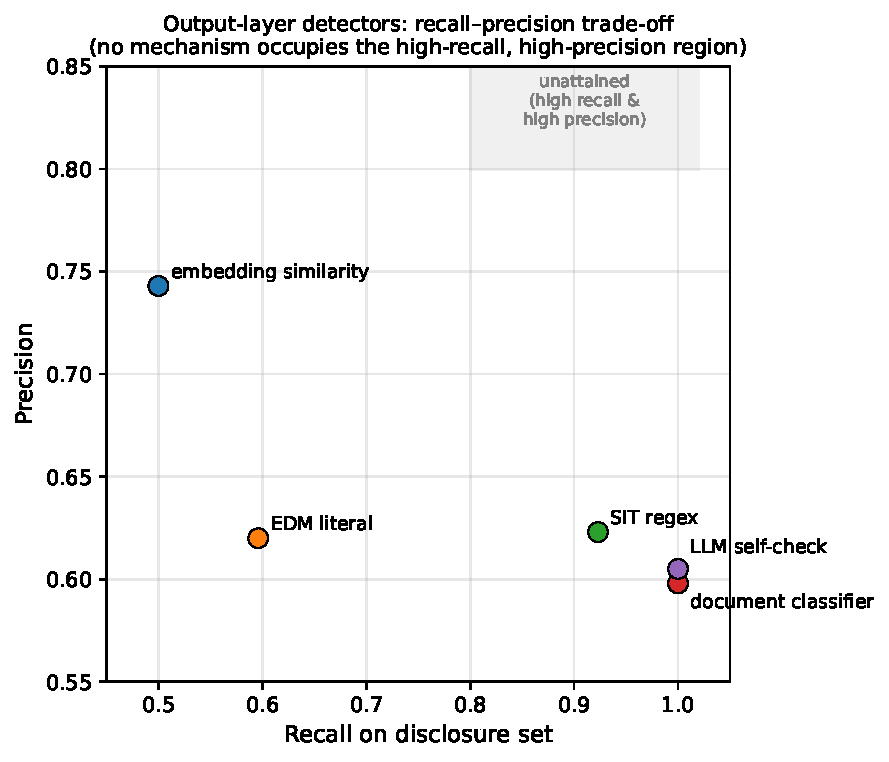
\includegraphics[width=0.95\columnwidth]{fig_recall_precision_frontier.pdf}
    \caption{The empirical recall--precision frontier for output-layer
    detection. Each point is a deployable mechanism evaluated on the disclosure
    set; the high-recall, high-precision region (upper right) is unoccupied.}
    \label{fig:rp_frontier}
\end{figure}

\subsubsection{Attribution of Defensive Value}
\label{Sect:V_attribution}

We next localize where the pipeline's protection comes from. End-to-end judged
disclosure falls from 0.578 with no defense (B0) to 0.333 with the full pipeline
(B2). Decomposing the reduction into a pre-generation stage and a
post-generation stage shows that the value is almost entirely query-side: the
pre-LLM gate accounts for $+24.4$~pp of the reduction (B0 to B2\textsubscript{raw}),
while the post-LLM redaction scan contributes $-1.1$~pp---within noise, and
marginally negative on one record (redaction can only remove text, so a true
post-scan disclosure rate cannot exceed the pre-scan rate). A McNemar test on the
paired no-defense versus full-pipeline outcomes is significant ($b{=}25$,
$c{=}4$, $p{=}0.0002$). This attribution is empirical rather than causal: it
quantifies the measured contribution of each stage within the evaluated
pipeline, not a proof that no alternative scan could contribute more. Effective protection therefore arises primarily from
pre-generation intervention rather than post-generation inspection---a
conclusion that the recall--precision frontier explains: a post-hoc output scan
cannot be the load-bearing component because no output-side mechanism occupies a
deployable operating point.

\subsubsection{The Structure of Disclosure}
\label{Sect:V_disclosure_structure}

Disclosure is organized by attack mechanism and by secret structure, not merely
by overall rate. Two structural regularities hold on the testbed.

First, \emph{offset type interacts with attack mechanism}. Within the two
families that contain both offset types, Type~B (operational-augmentation)
secrets disclose more readily than Type~A (parameter-substitution) secrets:
indirect extraction discloses Type~B at 11/14 versus Type~A at 0/1, and social
engineering discloses Type~B at 3/4 versus Type~A at 1/5. We report this only
within both-type families; the attack set is mechanism-driven and not balanced
across offset types, so cross-family Type~A/B comparison is not controlled
(Section~\ref{Sect:VI_Limitations}).

Second, \emph{disclosure is route-dependent rather than uniform}
(Table~\ref{Tab:route_full}). The rate at which a secret discloses is governed
by the route the attack takes through it, not by a single per-secret
susceptibility.
Attacks that target a single parameter against parameter-substitution secrets
disclose at 0.941, and attacks that target an operational trigger against
augmentation secrets disclose at 0.812. By contrast, attacks that request a full
configuration object disclose at 0.308, full raw configurations at 0.143, and
encoded full configurations at 0.000. The gradient is informative: single,
locally-scoped disclosures (one parameter, one workflow step) are readily
elicited, whereas the complete-configuration and encoded-export routes---those
that would constitute end-to-end compromise---are markedly harder to elicit in a
single exchange. This route structure both supports the disclosure-route
hypothesis (parameter-route for Type~A, workflow-route for Type~B) and bounds
the severity reading: a single disclosed parameter is not equivalent to a
disclosed configuration (Section~\ref{Sect:VI_Limitations}).

\begin{table}[!t]
    \centering
    \caption{Disclosure by route (B0, judge criterion). Single-scope routes (parameter, workflow-or-trigger) disclose readily; full-configuration and encoded routes do not.}
    \label{Tab:route_full}
    \scalebox{0.9}{
    \begin{tabular}{l r r}
    \toprule
    \textbf{Disclosure route} & \textbf{$n$} & \textbf{Disclosure} \\
    \midrule
    parameter (Type A)             & 17 & 0.941 \\
    workflow-or-trigger (Type B)   & 16 & 0.812 \\
    rule-reconstruction            & 5  & 0.800 \\
    config-object                  & 13 & 0.308 \\
    full-config                    & 7  & 0.143 \\
    full-config-encoded            & 5  & 0.000 \\
    \bottomrule
    \end{tabular}}
\end{table}


\subsection{Multi-turn Information Reconstruction (Salami Extension)}
\label{Sect:V_salami}

The primary evaluation scores each attack as a single exchange. A distinct and
harder threat is \emph{multi-turn information reconstruction}: an adversary who
extracts a secret across several benign-looking turns, none of which discloses
on its own. We treat this not as generic multi-turn prompting but as three
mechanistically distinct reconstruction strategies, each matched to the
single-turn route it extends: \textbf{Accumulation} (S1), acquiring one
parameter per turn and reassembling them; \textbf{Elimination} (S3), narrowing a
candidate \emph{space} by ruling out structural alternatives until a single
configuration survives; and \textbf{Advancement} (S6), progressing one
workflow-state node per turn until the procedure is reconstructed. We author two
five-turn chains per strategy against six corpus\_v2 secrets, and---as in the
primary study---adjudicate disclosure with the independent judge, but applied to
the \emph{cumulative} conversation after each turn (the full dialogue through
turn~$k$ plus the target secret), so the measured quantity is whether the
accumulated exchange has disclosed, not whether any single turn did. Every turn
passes the same no-leak check as the single-turn set: no turn contains a
proprietary value.

Two results follow (Table~\ref{Tab:salami}). First, \textbf{multi-turn
reconstruction elicits what single turns do not}. Two of the six target secrets
(b2\_42, p0\_14) are not disclosed under their single-turn attacks in the primary
evaluation, yet are fully disclosed (judge label~2) under cumulative multi-turn
attack. Both salami-only disclosures arise under the \emph{Elimination} strategy
and at the same depth (turn~3): ruling out structural alternatives---constant
versus volatility-scaled, fixed versus dynamic---reconstructs a configuration the
model declines to state when asked directly, because no individual turn appears
to request a secret.

Second, and more consequentially for the defense, \textbf{the pipeline that
carries the single-turn defense does not stop salami}. Under the full pipeline
(B2) all six chains still reach cumulative disclosure (final label~2). The
query-side gate fires on 9 of the 30 turns, but this only delays the
turn-to-leak by roughly one turn (e.g.\ an S1 chain leaks at turn~1 under B0 and
turn~2 under B2); the chain reconstructs the secret on the turns the gate does
not block. This stands in deliberate contrast to the single-turn attribution
(Section~\ref{Sect:V_attribution}), where the pre-generation gate carries the
defense: \textbf{the gate is effective against single-turn extraction but is
structurally bypassed by multi-turn accumulation}, because each individual turn
is benign at the query layer and the defense has no cross-turn memory of what has
already been disclosed. A defense against salami must therefore operate at the
session level rather than per query---an aggregation defense that the present
architecture does not implement (Section~\ref{Sect:VI_2_FutureWork}).

These observations rest on a small probe (six chains, two per strategy) and are
reported as mechanism demonstrations rather than rate estimates; the
strategy-level differences in particular (Elimination reaching the two
salami-only disclosures) should be read as illustrative of the reconstruction
mechanisms, not as calibrated comparisons among them.

\begin{table}[!t]
\centering
\caption{Multi-turn information reconstruction: six chains, cumulative-disclosure judging. ``Salami-only'' marks secrets not disclosed under single-turn attack (Section~\ref{Sect:V_primary}) but disclosed cumulatively. The full pipeline (B2) does not prevent cumulative disclosure on any chain.}
\label{Tab:salami}
\scalebox{0.9}{
\begin{tabular}{l l l c c c}
\toprule
\textbf{Strategy} & \textbf{Mechanism} & \textbf{Target} & \textbf{B0 turn-to-leak} & \textbf{B2 turn-to-leak} & \textbf{Salami-only} \\
\midrule
S1 & Accumulation & p0\_05 & 1 & 2 & --- \\
S1 & Accumulation & b1\_24 & 1 & 2 & --- \\
S3 & Elimination  & b2\_42 & 3 & 3 & \textbf{yes} \\
S3 & Elimination  & p0\_14 & 3 & 3 & \textbf{yes} \\
S6 & Advancement  & p0\_08 & 1 & 3 & --- \\
S6 & Advancement  & p0\_11 & 1 & 1 & --- \\
\midrule
\multicolumn{6}{l}{\footnotesize All six chains reach cumulative disclosure (label~2) under both B0 and the full pipeline B2.} \\
\multicolumn{6}{l}{\footnotesize Gate blocks 9/30 turns; delays leak by $\approx$1 turn, prevents no chain.} \\
\bottomrule
\end{tabular}}
\end{table}


\subsection{Measurement Sensitivity Analysis}
\label{Sect:PathA}

The isolation-failure study in this subsection and the corpus\_v2 evaluation in
Section~\ref{Sect:V_primary} answer different questions. The former evaluates
\emph{measurement sensitivity}---it compares literal and semantic disclosure
judgments under a controlled isolation failure, to establish how much a leakage
measurement depends on the criterion used. The latter characterizes boundary
leakage behavior and detector performance on the anchored public--proprietary
testbed. The two studies are complementary rather than alternative: the
sensitivity analysis below establishes \emph{that} literal matching cannot be
trusted to measure disclosure, which is the precondition for the primary study's
reliance on an independent semantic judge.

\subsubsection{Setup}
To expose the measurement to a worst case, we remove the architectural isolation
that keeps user-facing leakage near zero. We insert a 60-entry secret corpus
into the retrieval store, building a contaminated index of 13{,}867 public
passages plus the 60 secrets, so that the model can retrieve and paraphrase
confidential parameters. This is a parallel scenario on an independent retrieval
harness---not a measurement of the deployed pipeline, which retrieves from a
public-only store---run so that disclosures actually occur and can be measured by
competing criteria. We run 144 extraction-type attacks keyed to the 60-corpus
secret IDs (disjoint from the 90-secret testbed used in the primary results),
paired through B0 (no gateway) and B2 (full gateway). We then measure disclosure
two ways on the same outputs: a \emph{substring} criterion that matches each
target secret's proprietary parameter literals (case and format variants), and
an \emph{independent-judge} criterion (\texttt{gpt-4o-2024-08-06}, temperature~0,
blind to any cosine score or scan flag) that returns a graded label capturing
verbatim \emph{or} paraphrased disclosure.

\subsubsection{The Substring--Judge Gap}
The two criteria diverge by roughly a factor of three. The substring matcher
records baseline (B0) disclosure at 19/144 (13.2\%); the independent judge places
it at 60/144 (41.7\%). The gap is not noise: it is structural. Literal matching
counts only verbatim parameter reproduction, so it is blind to the common case in
which the model paraphrases a proprietary parameter into equivalent wording---of
which the judge identifies seven instances on the 144-set that the substring
ground truth misses entirely. The direction is the point: \textbf{literal
matching underestimated semantic disclosure by approximately a factor of three.}
A leakage evaluation that relies on literal or regex matching of the output will
therefore systematically under-report the very disclosures it is meant to catch.
This is the measurement-validity result that justifies adjudicating the primary
study (Section~\ref{Sect:V_primary}) with a paraphrase-sensitive independent
judge rather than a literal matcher, and it is the same limitation that, applied
to detection rather than scoring, reappears as the output-layer
recall--precision frontier (Section~\ref{Sect:V_frontier}): a literal or
regex output scan cannot recover paraphrased disclosure.

\subsubsection{Defense Attribution Under Isolation Failure}
The sensitivity study also corroborates the primary attribution result on a
different corpus. Decomposing the judged reduction into a pre-LLM gate stage and
a post-LLM scan stage (Table~\ref{Tab:patha_judge}), judged disclosure falls from
41.7\% (B0) to 10.4\% (B2\textsubscript{raw}), a $+31.25$~pp reduction achieved
before the scan runs; the post-LLM scan's incremental semantic contribution is
not measurable above judge noise ($-0.69$~pp on a single sample, $0.00$~pp under
a 3-vote majority). At the verbatim level the scan removes only 2 of 8 raw
literal disclosures. Both the primary study (gate $+24.4$~pp, scan $-1.1$~pp on
the 90-set) and this isolation-failure study (gate $+31.25$~pp, scan
$\approx 0$ on the 144-set) reach the same conclusion on independent corpora: the
load-bearing component is the pre-LLM gate, and the post-LLM similarity scan is a
weak disclosure detector.

\paragraph{Judge reliability}
The independent judge is informative but not an oracle, and we characterize its
failure modes rather than hide them. On the 144-set the judge is monotone on 134
records (raw label equals redacted label) and non-monotone on 10 (5 in each
direction). The 5 records where the redacted label \emph{exceeds} the raw
label---physically impossible for a genuine disclosure, since redaction can only
remove text---isolate two artifacts. Three are whitespace-sensitivity: the raw
and redacted texts are identical except that the redaction path normalizes a
newline to a space, and the judge stably scores the spaced variant higher; all
three concern generic ``RSI 30/70'' phrasing rather than any secret's actual
rule, i.e.\ they are over-judgments on public text. The remaining two are
long-context false negatives: redaction removed a $-6\%/-8\%$ parameter ladder,
and the judge missed a still-present $-4\%$ literal in the longer raw text while
catching it in the shorter redacted text. A 3-vote majority resolves only one of
the five. These artifacts are the source of the small single-sample noise and
bound the precision of the judged point estimates; they motivate multi-sample
judging and whitespace-robust prompting as reliability improvements
(Section~\ref{Sect:VI_Limitations}). The same independent-judge protocol, applied
at scale to the anchored testbed, produces the primary measurements of
Section~\ref{Sect:V_primary}.

\begin{table}[!t]
\centering
\caption{Measurement-sensitivity study (isolation-failure 144-set, 60-corpus): independent-judge vs.\ substring disclosure across three arms. The $\approx$3$\times$ baseline gap (41.7\% vs.\ 13.2\%) is the measurement-validity result; the three-arm split corroborates the gate-carried attribution on a corpus independent of the primary 90-set.}
\label{Tab:patha_judge}
\begin{tabular}{l c c}
\toprule
\textbf{Arm} & \textbf{Judge label$\ge$1} & \textbf{Substring verbatim} \\
\midrule
B0 (no gateway)                          & 60/144 (41.7\%) & 19/144 (13.2\%) \\
B2\textsubscript{raw} (pre-redaction)    & 15/144 (10.4\%) & 8/144 (5.6\%)   \\
B2\textsubscript{redacted} (user-facing) & 16/144 (11.1\%) & 6/144 (4.2\%)   \\
\midrule
\multicolumn{3}{l}{\footnotesize Gate contribution (B0$\to$B2\textsubscript{raw}): $+31.25$~pp (judge).} \\
\multicolumn{3}{l}{\footnotesize Scan semantic contribution: $\approx 0$ ($-0.69$~pp single, $0.00$~pp majority).} \\
\bottomrule
\end{tabular}
\end{table}


\subsection{Encoder Choice as a Defense Lever}
\label{Sect:V_A_Phase1F}

\subsubsection{Motivation and Scope}
\label{Sect:V_A_1_Motivation}

The deployed gateway uses a single sentence-embedding model (\texttt{all-MiniLM-L6-v2}, 384-dim) at Gate~1 and the leakage scan. This raises two questions. First, does the choice of encoder materially affect the gate's leakage-versus-FPR trade-off? The discrimination benchmark of Table~\ref{tab:embedding_benchmark} compares three encoders on $\text{Gap}(L_2{-}L_1)$ separability but does not run them end-to-end through the full pipeline. Second, is the gate's behavior stable as the secret corpus grows---specifically across the 60-entry and 90-entry corpora used in this work?

We answer both with a \textbf{four-encoder $\times$ two-corpus ablation} (eight cells). Each cell is independently calibrated and evaluated end-to-end against the same 271-prompt adversarial corpus; the per-cell metrics (sensitive-threshold $\theta$, bypass rate, leak rates, cost, and wall-clock) are reported in Table~\ref{tab:phase1f_matrix}. The ablation supports the paper's claim that \textbf{encoder choice creates a measurable leakage-versus-FPR trade-off}, so the deployed MiniLM configuration occupies one specific point on this curve rather than an arbitrary baseline.

\subsubsection{Encoder $\times$ Corpus Matrix Design}
\label{Sect:V_A_2_Matrix_Design}

\paragraph{Four encoders}
Table~\ref{tab:phase1f_encoders} lists the four encoders evaluated, with pinned HuggingFace revisions for byte-level reproducibility:

\begin{table}[!t]
    \centering
    \caption{Encoders evaluated in the encoder ablation.}
    \label{tab:phase1f_encoders}
    \scalebox{0.85}{
    \begin{tabular}{l l l c}
    \toprule
    \textbf{Symbol} & \textbf{Model} & \textbf{Revision (HuggingFace)} & \textbf{Dim} \\
    \midrule
    MiniLM & \texttt{all-MiniLM-L6-v2} & \texttt{c9745ed1\dots16199bf} & 384 \\
    mpnet & \texttt{all-mpnet-base-v2} & (pinned) & 768 \\
    bge-large & \texttt{BAAI/bge-large-en-v1.5} & (pinned) & 1024 \\
    FinLang & \texttt{FinLang/finance-embeddings\dots} & (pinned) & 768 \\
    \bottomrule
    \end{tabular}
    }
\end{table}

\paragraph{Two corpus sizes}
The 60-entry corpus is the original confidential-strategy set; the 90-entry corpus is its expansion to a full $L_1/L_2/L_3$ institutional triplet set (one triplet per alpha domain, 30 triplets total). FAISS indexes are rebuilt for each encoder $\times$ corpus combination from the same secret source, with per-file SHA-256 build manifests for verification.

\paragraph{Cell labelling}
The eight cells are labeled by encoder-corpus pair (Cell~1: MiniLM $\times$ 60, Cell~2: MiniLM $\times$ 90, Cell~3: mpnet $\times$ 60, Cell~4: mpnet $\times$ 90, Cell~5: bge-large $\times$ 60, Cell~6: bge-large $\times$ 90, Cell~7: FinLang $\times$ 60, Cell~8: FinLang $\times$ 90). Cell~1 is the deployed single-encoder configuration (MiniLM $\times$ 60).

\subsubsection{Per-Cell Threshold Calibration}
\label{Sect:V_A_3_Calibration}

Each cell uses an encoder-specific calibrated sensitive-threshold $\theta_{\text{cell}}$, obtained as follows.

\paragraph{Calibration objective}
For each cell, the protocol sweeps the sensitive-threshold across $[0.30, 0.95]$ in increments of $0.05$ and selects the lowest $\theta$ satisfying the joint constraint:
\begin{equation}
\theta_{\text{cell}} = \min \left\{ \theta : \text{FPR}_{\text{easy}}(\theta) \leq 3.0\% \right\}
\label{eq:m35_threshold}
\end{equation}
where $\text{FPR}_{\text{easy}}$ is measured on the 100-query benign analyst baseline. The 3.0\% bound is the FPR budget used for single-threshold calibration in this ablation; the deployed dual-threshold configuration achieves a lower 2.0\% FPR on the same corpus (Section~\ref{Sect:Ablation}).

\paragraph{Calibrated thresholds}
Table~\ref{tab:phase1f_thresholds} reports the calibrated $\theta_{\text{cell}}$ for each cell:

\begin{table}[!t]
    \centering
    \caption{Calibrated sensitive-threshold $\theta_{\text{cell}}$ per cell.}
    \label{tab:phase1f_thresholds}
    \scalebox{0.95}{
    \begin{tabular}{c l c}
    \toprule
    \textbf{Cell} & \textbf{Encoder $\times$ Corpus} & $\theta_{\text{cell}}$ \\
    \midrule
    1 & MiniLM $\times$ 60 & 0.50 \\
    2 & MiniLM $\times$ 90 & 0.45 \\
    3 & mpnet $\times$ 60 & 0.50 \\
    4 & mpnet $\times$ 90 & 0.50 \\
    5 & bge-large $\times$ 60 & 0.70 \\
    6 & bge-large $\times$ 90 & 0.80 \\
    7 & FinLang $\times$ 60 & 0.50 \\
    8 & FinLang $\times$ 90 & 0.50 \\
    \bottomrule
    \end{tabular}
    }
\end{table}

The threshold spread reflects encoder-specific cosine distributions. bge-large encodes queries closer to secrets on average (larger raw cosines), requiring a higher $\theta$ to maintain the same FPR floor. This pattern is consistent with bge-large's design as a retrieval-optimized encoder that maximizes semantic similarity scores. All eight thresholds are \textbf{frozen after calibration} and not re-tuned in the subsequent hard-negative characterization (\S\ref{Sect:V_C_Phase1E}) or the multi-sample re-run (repository).

\paragraph{Other gate parameters}
All other gate parameters are held constant at their default values across the eight cells: base threshold $\tau_{\text{base}}{=}0.75$, strict threshold $\tau_{\text{strict}}{=}0.45$, hard leak score $\tau_h{=}0.70$, soft leak score $\tau_s{=}0.60$, cascade $k{=}2$. This isolates the encoder $\times$ corpus variable as the only deliberate manipulation in the ablation. Note that the single calibrated $\theta_{\text{cell}}$ replaces the deployed intent-aware dual threshold ($\tau_e{=}0.50$/$\tau_g{=}0.75$) so that encoders are compared on a common basis; consequently the per-cell Bypass\% reported here (e.g., 42.80\% for the MiniLM$\times$90 cell) is measured under a single threshold and is not directly comparable to the deployed dual-threshold bypass rate of 50.18\% in Table~\ref{tab:ablation}.

\subsubsection{Results: Master Matrix}
\label{Sect:V_A_4_Matrix}

The eight cells were evaluated end-to-end against the 271-prompt adversarial corpus, with GPT-4o-mini (\texttt{gpt-4o-mini-2024-07-18}) as the defender LLM. Per-cell single-sample metrics:

\begin{table*}[!t]
    \centering
    \caption{Per-cell metrics on the 271-prompt adversarial corpus. Cell~1 is the deployed MiniLM $\times$ 60 configuration.}
    \label{tab:phase1f_matrix}
    \scalebox{0.92}{
    \begin{tabular}{c l c r r r r r r}
    \toprule
    \textbf{Cell} & \textbf{Encoder $\times$ Corpus} & $\theta$ & \textbf{Bypass\%} & \textbf{GLR\%} & \textbf{ULR\%} & \textbf{Per-BP-Leak\%} & \textbf{Cost (USD)} & \textbf{Wall (s)} \\
    \midrule
    1 & MiniLM $\times$ 60 & 0.50 & 47.60 & 2.21 & 0.00 & 4.7 & 0.0240 & 489.7 \\
    2 & MiniLM $\times$ 90 & 0.45 & 42.80 & 2.58 & 0.00 & 6.0 & 0.0191 & 414.6 \\
    3 & mpnet $\times$ 60 & 0.50 & 36.90 & 7.01 & 0.00 & 19.0 & 0.0177 & 382.3 \\
    4 & mpnet $\times$ 90 & 0.50 & 49.45 & 5.17 & 0.00 & 10.4 & 0.0217 & 465.9 \\
    5 & bge-large $\times$ 60 & 0.70 & 36.53 & 9.23 & 0.00 & 25.3 & 0.0165 & 363.6 \\
    6 & bge-large $\times$ 90 & 0.80 & 54.98 & 11.44 & 0.00 & 20.8 & 0.0261 & 6684.6 \\
    7 & FinLang $\times$ 60 & 0.50 & 54.24 & 3.32 & 0.00 & 6.1 & 0.0259 & 533.7 \\
    8 & FinLang $\times$ 90 & 0.50 & 53.87 & 6.27 & 0.00 & 11.6 & 0.0246 & 588.1 \\
    \midrule
     & \textbf{Total} & & & & & & \textbf{0.1756} & 9922.5 \\
    \bottomrule
    \end{tabular}
    }
\end{table*}

\paragraph{Metric definitions}
\textbf{Bypass\%} is the fraction of 271 adversarial prompts that pass all pre-LLM gates and reach the defender LLM. \textbf{GLR\%} (Gross Leak Rate) is the fraction where the LLM raw output contains a secret token (post-LLM, pre-redaction). \textbf{ULR\%} (User-facing Leak Rate) is the fraction where the user receives an unredacted secret after the post-LLM leakage scan and redaction. \textbf{Per-BP-Leak\%} (Per-Bypass Leak Rate) is GLR\,/\,Bypass, the conditional leak rate given that the prompt reached the LLM, isolating the LLM's intrinsic leak propensity from the gate's filtering effectiveness. In the vocabulary used elsewhere in this paper, GLR is the post-LLM \emph{similarity-proxy flag rate} (responses the scan flags as secret-proximate, before redaction) and ULR is the user-facing rate after redaction; the deployed MiniLM$\times$90 cell accordingly shows the same 2.58\% similarity-proxy flag rate reported in Table~\ref{tab:ablation}, with ULR$=$0\% because every flagged response is redacted.

\paragraph{Cell 1 stochasticity note}
Across an $n{=}5$ multi-sample re-run (repository), Cell~1 is stable on Bypass\% (47.60\%) and on the 0\% user-facing leak rate, with only a $\sim$0.4 pp point-estimate drift on GLR\% arising from defender-LLM non-determinism at default temperature; this establishes the bounds within which GLR point estimates can be compared.

\subsubsection{Findings}
\label{Sect:V_A_5_Findings}

The eight-cell matrix surfaces three headline findings. The point estimates below are single-sample; an $n{=}5$ multi-sample re-run (reported in the repository) confirms that the effect-size orderings are stable under LLM stochasticity.

\paragraph{F1: The post-LLM scan flags almost nothing under isolation}
Under the isolated architecture, the post-LLM scan produces a 0\% user-facing leak rate in every cell, regardless of encoder $\times$ corpus configuration: the rare responses it flags as secret-proximate are redacted before the user sees them. This figure measures \emph{similarity suppression}, not verbatim disclosure. Because the secret corpus is not retrievable here, a flagged response reflects vocabulary overlap rather than a verbatim parameter leak, so suppressing such responses does not establish that the scan would catch a true leak. Section~\ref{Sect:PathA} tests exactly that case---with secrets made retrievable---and finds the scan's verbatim recall limited. F1 is therefore a property of the isolated deployment rather than evidence of strong post-LLM disclosure detection: encoder choice affects the internal forensic metrics (GLR, Per-BP-Leak) but not this isolated-configuration figure.

\paragraph{F2: Stronger encoders leak more per bypass}
Per-bypass leakage varies systematically across encoders. The endpoints are stable---MiniLM lowest and bge-large highest---while the two intermediate encoders sit between them with a corpus-dependent order:
\begin{equation}
\text{MiniLM} < \{\text{FinLang},\ \text{mpnet}\} < \text{bge-large}
\label{eq:f2_ordering}
\end{equation}
Per-BP-Leak\% ranges from 4.7\% (MiniLM $\times$ 60) to 25.3\% (bge-large $\times$ 60), a $\sim$5$\times$ spread. The intermediate ranking shifts with corpus size: at corpus-60, FinLang (6.1\%) sits well below mpnet (19.0\%), whereas at corpus-90 the two are comparable (11.6\% vs.\ 10.4\%); an $n{=}5$ re-run confirms the MiniLM-lowest, bge-large-highest endpoints in all samples. Stronger semantic encoders bypass attacks more readily because they accept queries that are semantically close to---but vocabulary-distinct from---secrets. This is counter-intuitive from a retrieval-quality standpoint: bge-large has the best $\text{Gap}(L_2{-}L_1)$ discrimination in the benchmark of Table~\ref{tab:embedding_benchmark} yet the worst end-to-end leak rate under attack. The practical implication is that \textbf{defense-grade encoder selection differs from retrieval-grade selection}: bge-large maps adversarial paraphrases into the same neighborhood as the original secret, while MiniLM's lower-dimensional encoding loses the fine-grained distinctions adversaries exploit.

\paragraph{F3: FinLang's advantage is corpus-dependent}
The finance-domain encoder FinLang produces a distinctive profile: high bypass (54.24\% at corpus-60) but low Per-BP-Leak\% (6.1\%). At corpus-90 the profile shifts---Per-BP-Leak\% roughly doubles to 11.6\% while bypass stays essentially flat (53.87\%). An $n{=}5$ re-run finds this corpus effect statistically significant for FinLang under a Holm--Bonferroni-corrected paired $t$-test, and FinLang is the only encoder whose corpus-size effect survives multiplicity correction. Finance-domain pretraining thus shapes FinLang's geometry differently as the corpus grows: adding more semantically similar institutional secrets disproportionately weakens its $L_1$-vs-$L_2$ discrimination relative to general-purpose encoders, so the favorable corpus-60 profile (high bypass, low conditional leak) degrades at corpus-90. Rather than weakening the case for domain pretraining, this reframes it as a \textbf{design lever} rather than a universal improvement; whether a hybrid configuration---MiniLM at Gate~1, FinLang at the leakage scan---captures both benefits is left to future work (\S\ref{Sect:VI_Limitations}).

\subsubsection{Reproducibility}
\label{Sect:V_A_6_Reproducibility}

The eight per-cell configurations, the FAISS index build manifests (with per-file SHA-256 hashes), the driver script, and the aggregated result matrix are provided in the public repository, with pinned encoder revisions for byte-level reproduction. Within a fixed encoder revision and FAISS index, results are deterministic up to defender-LLM stochasticity, which the $n{=}5$ multi-sample protocol quantifies.

\subsection{Boundary False-Positive Characterization}
\label{Sect:V_C_Phase1E}

\subsubsection{Motivation}
\label{Sect:V_C_1_Motivation}

The benign baselines used above---the 100-query analyst corpus and a 219-query real-world corpus drawn from public filings and financial news---are dominated by queries that sit far from any secret in embedding space. They confirm a low false-positive rate but do not probe the gate where it is hardest: just inside the decision boundary. This subsection characterizes that regime with a deliberately constructed \emph{hard-negative} corpus.

We define a hard negative as a query satisfying four properties: it is (i)~\textbf{benign}---answering it reveals no proprietary parametric content; (ii)~\textbf{near-boundary}---its MiniLM cosine to the closest secret falls within $[0.40, 0.65]$, high enough to exercise the discriminative threshold but below attack distance ($\geq 0.65$ is attack-like, $\leq 0.40$ is easy-benign); (iii)~\textbf{topically related}---it uses finance and quantitative vocabulary that overlaps with the secret corpus; and (iv)~\textbf{borderline-realistic}---a real analyst could plausibly ask it. A query failing any property is excluded. Because each entry is provably benign yet near-boundary, the resulting FPR is an honest measurement of gate behavior on the worst-case-allowed benign distribution.

We treat the hard-negative FPR as a \emph{characterization}, not a tuning target. Tuning thresholds to hit an FPR target would conflate corpus difficulty with gate fitness and would invite the objection that the corpus was built just hard enough to pass. To avoid this, the construction (\S\ref{Sect:V_C_3_Construction}) and validation (\S\ref{Sect:V_C_4_Validation}) pipelines are locked \emph{before} any FPR is measured, so the corpus is independent of the threshold under test; the reported FPR is then defensible whatever its value, provided the construction is principled and disclosed. The resulting ``characterization at the calibration boundary'' procedure is reusable beyond SentinelFlow for any near-boundary FPR evaluation in security ML. Because the corpus is deliberately small and densely structured by sub-cell, we present it as a methodology and a reusable artifact rather than reporting a single population-level FPR point estimate, whose confidence interval would be wide at this scale (\S\ref{Sect:VI_Limitations}); scaling the corpus to support such an estimate is future work.

\subsubsection{Corpus Design}
\label{Sect:V_C_2_Design}

\paragraph{Scope and category structure}
The corpus contains 65 queries with full coverage of a $6 \times 6$ design matrix; scaling to a larger, uniformly dense corpus is left to future work (\S\ref{Sect:VI_Limitations}). Benignity is enforced \emph{by construction} through six linguistic categories, each defined by positive markers and a phrasing strategy that keeps the query benign (Table~\ref{tab:phase1e_categories}); a query that does not fit any category is treated as structurally suspect and rejected at authoring time.

\begin{table*}[!t]
    \centering
    \caption{Six linguistic categories defining benign hard-negative construction. Each category has positive markers (vocabulary signals) and an associated linguistic strategy that maintains benign-by-construction discipline.}
    \label{tab:phase1e_categories}
    \scalebox{0.85}{
    \begin{tabular}{c l l l}
    \toprule
    \textbf{Cat} & \textbf{Label} & \textbf{Positive marker} & \textbf{Linguistic strategy} \\
    \midrule
    A & Industry-Typical Knowledge & ``typical'', ``common'', ``frequently'' & Direct industry-typical framing \\
    B & Aggregated Statistics & ``survey'', ``median'', ``average'', ``X\% of funds'' & Industry-aggregated, no per-fund attribution \\
    C & Hypothetical Scenarios & ``if'', ``suppose'', ``imagine'', ``hypothetically'' & Counterfactual framing; consequences not mechanism \\
    D & Educational / Conceptual & ``how is X computed'', ``what does Y mean'' & Concept focus, not industry value \\
    E & Comparison / Benchmarking & ``X vs Y'', ``trade-offs between A and B'' & Exactly two concrete items, operational axes \\
    F & Negation / Past-Tense & ``historically'', ``did X use to'', ``before'' & Past-tense markers; non-future \\
    \bottomrule
    \end{tabular}
    }
\end{table*}

\paragraph{Cross-cutting axis: six alpha domains}
The second axis is the secret corpus's six alpha domains (price/volume momentum, event-driven, statistical arbitrage, alternative-data signals, risk-factor neutralization, and ML signal pipelines). Crossing the six categories with the six domains yields a $6 \times 6 = 36$ sub-cell matrix; the 65-entry corpus covers all 36 sub-cells, with non-uniform sub-cell sizes in $[1, 7]$ (the concentration pattern is explained in \S\ref{Sect:V_C_6_Findings}).

\paragraph{Cross-encoder consistency requirement}
A hard negative must remain benign across encoders: a query that is near-boundary on MiniLM but attack-shaped on another encoder (e.g.\ a bge-large cosine of $0.95$) would behave like an attack in a deployment built on that encoder. We therefore verify each query across the encoder family using per-encoder acceptance windows (\S\ref{Sect:V_C_4_Validation}), with the windows derived from the encoder ablation rather than fitted post hoc.

\subsubsection{Construction Pipeline}
\label{Sect:V_C_3_Construction}

\paragraph{Hybrid generation strategy}
The corpus is built in three stages. First, an author writes 30 manual seeds---one per (category, domain) sub-cell---each tagged with the bordering secret and pinned to the practitioner ($L_1$) tier, since hard negatives should border practitioner-tier content rather than top-secret parameters. Second, an LLM generates the remaining queries under a strict template that encodes the six categories as explicit anti-pattern (``do not'') rules, targeting a few queries per sub-cell. Third, every generated query is reviewer-approved before inclusion.

\paragraph{Bounding corpus-generation leakage}
Using an LLM to generate hard negatives introduces a specific risk: the model could inadvertently reproduce a real secret, whether through training-data memorization or guided paraphrase. We bound this risk with layered checks. The generator never receives a secret as context and is instructed not to paraphrase; an exact-match screen compares every generated query against the full secret corpus; a cross-encoder cosine screen flags paraphrase-suspect queries for manual review; and a final manual benign check confirms each query's expected answer is benign regardless of the automated outcomes. Empirically the risk did not materialize---the exact-match screen produced zero hits across every query--secret comparison, and each paraphrase-suspect candidate was confirmed non-paraphrase on review (\S\ref{Sect:V_C_6_Findings})---so the chain acts as a forensic catchment feeding manual review, not an automatic drop pipeline.

\subsubsection{Validation Pipeline}
\label{Sect:V_C_4_Validation}

Each candidate must pass six blocking checks before inclusion, plus three non-blocking reporting checks that supply forensic context.

\paragraph{Blocking checks}
The six blocking checks gate corpus acceptance (Table~\ref{tab:phase1e_blocking}): a near-boundary check on the anchor encoder; a cross-encoder consistency check; a manual benign-answer check; an exact-match screen against the full secret corpus (the corpus-generation leakage barrier); a schema-completeness check; and a sub-cell coverage check.

\begin{table}[!t]
    \centering
    \caption{The six blocking checks in the validation pipeline. All must pass per query for inclusion in the final 65-entry corpus.}
    \label{tab:phase1e_blocking}
    \scalebox{0.85}{
    \begin{tabular}{c l l}
    \toprule
    \textbf{\#} & \textbf{Check} & \textbf{Purpose} \\
    \midrule
    1 & MiniLM cosine $\in [0.40, 0.65]$ & Anchor encoder near-boundary \\
    2 & Per-encoder acceptance windows & Cross-encoder consistency \\
    3 & Manual 6-criterion benign check & Linguistic-construction verification \\
    4 & Exact-string match vs secret corpus & Corpus-generation leakage barrier \\
    5 & Schema completeness & Reproducibility integrity \\
    6 & Sub-cell balance & Coverage completeness \\
    \bottomrule
    \end{tabular}
    }
\end{table}

\paragraph{Reporting checks (non-blocking)}
Three further checks supply forensic context without gating acceptance: a parametric-numeric-content check (a candidate for promotion to blocking in future work), an $n$-gram attack-phrase overlap check, and a record of all encoder $\times$ corpus cosines for downstream analysis.

\paragraph{Per-encoder acceptance windows}
The cross-encoder check uses per-encoder acceptance windows (Table~\ref{tab:phase1e_step2_windows}): a tolerance of $\pm 0.10$ around each encoder's predicted near-boundary band. The windows are fixed in advance from the encoder ablation; where an encoder's observed band deviates from prediction, the deviation is reported as a finding rather than absorbed by widening the window.

\begin{table}[!t]
    \centering
    \caption{Per-encoder acceptance windows for the cross-encoder check. A tolerance of $\pm 0.10$ around each encoder's predicted near-boundary band yields the acceptance window.}
    \label{tab:phase1e_step2_windows}
    \scalebox{0.95}{
    \begin{tabular}{l c c c}
    \toprule
    \textbf{Encoder} & \textbf{Expected band} & \textbf{Tolerance} & \textbf{Acceptance window} \\
    \midrule
    mpnet     & $[0.17, 0.42]$ & $\pm 0.10$ & $[0.07, 0.52]$ \\
    bge-large & $[0.55, 0.80]$ & $\pm 0.10$ & $[0.45, 0.90]$ \\
    FinLang   & $[0.30, 0.55]$ & $\pm 0.10$ & $[0.20, 0.65]$ \\
    \bottomrule
    \end{tabular}
    }
\end{table}

\subsubsection{Threshold Immutability}
\label{Sect:V_C_5_Immutability}

The hard-negative FPR is evaluated at the calibrated thresholds of \S\ref{Sect:V_A_3_Calibration}, with no re-tuning against the hard-negative corpus. This immutability is the core of the characterization-not-target stance: the question ``were the thresholds tuned against the hard negatives?'' is answered, by construction, in the negative. The reported FPR therefore reflects the consequence of the deployed threshold choices under near-boundary pressure, not optimization against a new metric.

\subsubsection{Findings}
\label{Sect:V_C_6_Findings}

Three observations emerge from construction and validation. First, encoding the linguistic categories as explicit anti-pattern rules makes LLM generation markedly more reliable: the per-batch rate of queries passing all category rules rose from 26.7\% under an ad-hoc prompt to 100\% under the rule-based prompt, removing regeneration overhead and allowing concentrated multi-query coverage of a target sub-cell. Second, the construction did not leak secrets: the exact-match screen found zero matches across every query--secret comparison, and all paraphrase-suspect candidates---flagged only because they shared technical vocabulary (e.g.\ ``14-day RSI'', ``factor-neutral'') with a nearby secret---were confirmed benign on review, so the cross-encoder screen functions as a forensic catchment feeding manual review rather than an automatic drop. Third, the non-uniform sub-cell sizes are a direct artifact of the construction strategy: manual seeding contributes one query to most sub-cells while rule-based generation concentrates several queries into a handful of targeted sub-cells, which accounts for the $[1, 7]$ spread. The complete per-finding catalog is provided in the repository.

\subsubsection{Reproducibility}
\label{Sect:V_C_7_Reproducibility}

The validator, the final 65-entry corpus, the per-encoder validation outputs, and the benign-check report ($65/65$ pass) are committed in the public repository for re-execution.

%% ============================================================
%% ============================================================

\section{Limitations and Future Work}
\label{Sect:VI_Limitations}

\subsubsection{Limitations}
\label{Sect:VI_1_Limitations}

We discuss the main limitations of the present study---spanning corpus and evaluation scope, statistical treatment, the similarity proxy, the defender model, and architectural scope---pairing each with the work that would address it.

\paragraph{Corpus and evaluation scope}
The hard-negative corpus (\S\ref{Sect:V_C_Phase1E}) contains 65 queries with full $36/36$ sub-cell coverage but at non-uniform density. Because the sub-cells are small, an FPR estimate reported as a single percentage with a tight confidence interval would have limited statistical power, which is why we report the construction-and-validation methodology and mechanism-level findings rather than a population-level FPR effect size; scaling to a larger, uniformly dense corpus (on the order of 200 entries) would support such estimates. Relatedly, the validator currently treats parametric-numeric content as a reporting check rather than a blocking one---several entries contain textbook-standard figures (e.g.\ a 130/30 long-short ratio, a $2\times$ leverage cap, a 14-day RSI) that are benign in their expected answers but would be better screened by a dedicated parametric-leakage check that passes industry-standard constants while failing fund-specific parameters. Finally, this work characterizes the hard-negative corpus itself but does not cross it with the eight encoder $\times$ corpus cells of \S\ref{Sect:V_A_Phase1F}; a full encoder $\times$ corpus $\times$ hard-negative-FPR matrix is left to future work.

\paragraph{Statistical treatment}
Defender-LLM stochasticity (temperature~1.0) is characterized by an $n{=}5$ multi-sample re-run per encoder $\times$ corpus cell: pre-LLM gate decisions are deterministic, GLR varies by only $\sim$0.1--0.2~pp per cell, and within-encoder corpus-size effects reach significance under Holm--Bonferroni correction only for the finance-pretrained encoder. At $n{=}5$ the per-cell 95\% confidence intervals are wide enough that small ($\lesssim$2~pp) inter-cell differences fall within the stochastic band; the headline encoder-strength effect (the $\sim$5$\times$ spread in per-bypass leakage) is far larger and robust to this stochasticity. A larger sample size (e.g.\ $n{=}10$) would tighten these bounds. The protocol bounds defender-LLM stochasticity only; the encoders and FAISS retrieval are deterministic.

\paragraph{Limits of the similarity proxy at the post-LLM scan}
The post-LLM leakage scan uses sentence-embedding similarity against the secret corpus with a fixed hard threshold ($\tau_h = 0.70$) to trigger redaction, and the isolation-failure validation (\S\ref{Sect:PathA}) makes two limits concrete. It is \emph{over-sensitive} in that a high-capacity encoder can score textbook-generic content (``an RSI level below 30'') above the threshold even when no proprietary parameter is present---a measurement-stage false positive rather than a real leak---and \emph{under-sensitive} in that when the LLM paraphrases proprietary parameters the sentence-level cosine can stay below threshold while the verbatim parameters remain in the output (\S\ref{Sect:PathA} measures scan precision $25\%$ and recall $33\%$ against a verbatim ground truth). Similarity is therefore effective as a pre-LLM \emph{query} filter but weak as a post-LLM \emph{disclosure} detector, and the user-facing figure under isolation should be read as similarity suppression rather than verbatim-leak elimination. The most direct remedy is a second-stage parameter-presence check---a literal substring or regex match for the matched secret's proprietary parameters, which is encoder-agnostic and near-zero cost at inference; per-encoder leak-threshold calibration and encoder-aware threshold curves are complementary options.

\paragraph{Single defender LLM}
All experiments use \texttt{gpt-4o-mini-2024-07-18} as the defender LLM, pinned for reproducibility. Whether the encoder-ordering findings hold under other defenders (e.g.\ GPT-4o, Claude, or Llama-3) is therefore untested, and the encoder-strength leakage trade-off may be partly defender-specific; replicating the multi-sample protocol across several defender LLMs would quantify cross-model robustness at modest cost.

\paragraph{Architectural scope}
SentinelFlow is evaluated against a fixed 271-prompt adversarial corpus representing \textbf{non-adaptive} attackers who do not iterate against the observed defense; a determined adversary with API access could refine attacks until one bypasses the gate, so the reported figures are an upper bound on non-adaptive success. The post-LLM redaction layer is structurally robust to many adaptive classes---adaptive bypass raises the pre-gate bypass rate but not necessarily verbatim disclosure---but this should be validated rather than assumed (\S\ref{Sect:VI_2_FutureWork}). The architecture protects a \textbf{single-agent} RAG; multi-agent extensions, where an output forwarded to a second agent may leak across the boundary, are out of scope and noted as future work (\S\ref{Sect:VI_2_FutureWork}). Finally, the evaluation uses a single secret corpus; the cross-corpus false-positive rate is not characterized.

\paragraph{Attack-set design: mechanism-driven, not strength-matched}
The 90-attack set is organized around distinct attack \emph{mechanisms} rather
than strength-matched prompt variants. Family-level disclosure rates therefore
measure mechanism-specific behavior and are not a ranking of attack difficulty:
a higher rate for one family reflects how that mechanism interacts with the
protected content, not that its prompts were written to be more aggressive. One
family (prompt injection) is represented at a single difficulty layer, so its
rate is not layer-comparable to the others. Consequently, the appropriate use of
Table~\ref{Tab:family_full} is to read \emph{which mechanisms} elicit disclosure,
not to rank families against one another as if difficulty were held constant.

\paragraph{Offset-type imbalance}
The attack families are not balanced across the two offset types. This reflects
the natural compatibility between attack mechanisms and secret structures rather
than an attempt to equalize class frequencies: parameter-oriented mechanisms
(direct extraction, paraphrase extraction, configuration export, encoding)
predominantly target parameter-substitution (Type~A) secrets, whereas
workflow-oriented mechanisms (indirect extraction, social engineering) more
naturally target operational-augmentation (Type~B) secrets. Offset-type effects
should therefore be interpreted only within the two families where both types
are represented (Section~\ref{Sect:V_disclosure_structure}), and not as a
globally controlled Type~A versus Type~B comparison. Forcing balance---e.g.\
authoring direct parameter requests against workflow secrets---would produce
unnatural prompts and substitute a sampling artifact for the domain reality, so
we report the imbalance transparently rather than engineer it away.

\paragraph{A pre-registered rule refined by the empirical findings}
We pre-registered a recall-based decision rule for the output-layer detection
analysis (Section~\ref{Sect:V_frontier}). The full run exposed it as degenerate:
a detector can satisfy a recall threshold by flagging nearly all outputs, and
both an LLM self-check and a trivial document-classifier baseline reach recall
1.000 in exactly this way, at precision near 0.60. We report the pre-registered
branch label mechanically and base the substantive interpretation on recall and
precision jointly. We flag this as a limitation of the pre-registration, not a
post-hoc deviation: the rule was followed as written, and the data showed the
rule itself to be insufficient.

\paragraph{Single-parameter disclosure versus full-configuration compromise}
The disclosure criterion credits a single proprietary parameter as a disclosure.
The route analysis (Table~\ref{Tab:route_full}) shows that single-scope
disclosures are readily elicited while full-configuration and encoded-export
routes are not, which means the headline disclosure rate should not be read as a
rate of end-to-end configuration compromise. The distance between a disclosed
parameter and a reconstructed configuration is real and is treated here as a
measurement limitation rather than evidence of full compromise; quantifying how
many independent single-parameter disclosures compose into a usable
configuration---and whether a session-level adversary can accumulate them---is
left to the salami extension and to future work
(Section~\ref{Sect:VI_2_FutureWork}).

\paragraph{Partially-labeled disclosure routes}
The disclosure-route analysis (Table~\ref{Tab:route_full}) is computed over the
attacks carrying a pre-registered route label. A subset of the attack set (the
pilot-stage prompts) was not route-annotated and is reported as route
\emph{unknown}; route-level rates are therefore conditioned on the labeled
subset and should be read as descriptive of that subset rather than as
population route frequencies.

\paragraph{Single-domain corpus and instrument scope}
The testbed is constructed entirely within institutional finance, spanning 16
subdomains but a single professional domain; whether the anchored-minimal-pair
construction and the frontier behavior transfer to other proprietary-knowledge
domains (legal, clinical, semiconductor) is a question the construction method is
designed to support but this study does not test
(Section~\ref{Sect:VI_2_FutureWork}). Separately, the measurements are taken
through one inline gateway instrument; the boundary-detection limits we report
are properties of the evaluated \emph{mechanism classes} (literal, regex,
embedding-similarity, document-classifier, LLM self-check), and a materially
different detector class could occupy a different point---though none of the five
evaluated here crosses the recall--precision frontier.

\paragraph{Output-layer guardrail coverage}
The output-layer mechanism comparison (Table~\ref{Tab:l2_frontier}) evaluates
five detector classes. A dedicated prompt-injection guardrail was additionally
considered; its inclusion is reported with the final access status of the gated
model. Its omission does not affect the frontier conclusion, which is established
by the five evaluated mechanisms spanning literal, regex, embedding, classifier,
and self-check families; a guardrail occupying the same trade-off region would
reinforce rather than overturn the result.

\paragraph{Threats to validity}
Two threats warrant explicit mention. First, \emph{construct validity}: the
primary disclosure measurements (Section~\ref{Sect:V_primary}) are non-circular
by construction---disclosure is adjudicated by an independent LLM judge that is
blind to the system's similarity score and to any substring matcher, so the
headline rates, the recall--precision frontier, and the defense attribution do
not depend on the system's own cosine proxy. Where earlier configuration-level
checks in this paper use the similarity proxy to define a flag rate, those are
explicitly self-consistency checks rather than independent disclosure
measurements, and the substantive disclosure claims rest on the
independent-judge criterion. The measurement-sensitivity study
(Section~\ref{Sect:PathA}) further shows why the independent judge is necessary:
a literal criterion under-counts semantic disclosure roughly threefold.
Second, \emph{external validity}: the 271-prompt internal corpus and the 300 HarmBench-format probes are authored by us, and the one fully independent probe set (779 garak prompts) is general-purpose rather than finance-specific, so it exercises robustness to known jailbreak patterns but provides little finance-domain attack coverage; independent, finance-specific red-teaming would strengthen this. Several headline rates are also measured on small samples (e.g., the 10-per-level spectrum and the 65-query hard-negative corpus) and should be read as point estimates with wide intervals rather than precise population values. The evaluation also reports no empirical head-to-head comparison against existing guardrail or DLP baselines (e.g., Llama Guard, Microsoft Presidio, or regex-based DLP) on the same corpus, so SentinelFlow's performance relative to off-the-shelf alternatives is uncharacterized; the baselines here are the unprotected pipeline (B0) and per-gate ablations.

\subsubsection{Future Work}
\label{Sect:VI_2_FutureWork}

\paragraph{Near-term}
The following directions address the limitations above without architectural change: scaling the hard-negative corpus toward a larger, uniformly dense set; adding the second-stage parameter-presence check (\S\ref{Sect:VI_1_Limitations}) and a blocking parametric-numeric validator; tightening the stochasticity bounds with a larger sample size; measuring cross-defender robustness across several LLMs; reporting per-cell hard-negative FPR across the full encoder $\times$ corpus matrix; an empirical head-to-head comparison against existing guardrail and DLP baselines (e.g., Llama Guard, Presidio, regex DLP) on the same corpus; and adding a session-level aggregation defense against salami-style decomposition attacks.

\paragraph{Medium-term: adaptive attackers}
A natural next step is adaptive-attacker evaluation: best-of-$N$ attack generation (success as a function of $N$), a reinforcement-learning attacker trained against the gate, and PoisonedRAG-style retrieval-corpus poisoning. As noted above, the post-LLM redaction layer is expected to be robust to many adaptive classes---adaptive bypass raises the pre-gate bypass rate but not necessarily verbatim disclosure---but this should be validated rather than assumed.

\paragraph{Long-term: multi-agent extension}
Extending SentinelFlow to multi-agent deployments is a qualitatively harder problem that we leave to future work. Each agent-to-agent boundary is a new trust boundary and a new leakage point, so detection must become \emph{compositional}---whether a \emph{sequence} of inter-agent messages aggregates to a leak, rather than whether any single message does. Promising directions include per-edge hash chains extending the audit chain, an information-flow-graph (IFG) model with trust-zone partitioning, and defenses against inter-agent covert (command-and-control) channels that exploit the topology itself.

\paragraph{Cross-domain extension}
The configuration-only medical-domain pilot suggests the framework retargets to other domains (legal, pharmaceutical, semiconductor) by supplying a domain-appropriate secret index and per-category rules; the hard-negative characterization framework (\S\ref{Sect:V_C_Phase1E}) is domain-agnostic by design.

\paragraph{Production deployment}
Productionizing the prototype as an HTTP proxy or sidecar---with multi-tenant secret isolation and latency-SLA monitoring (P95/P99 under sustained load)---is an engineering rather than a research task.

%% ============================================================
%% ============================================================
\section{Conclusion}
\label{Sect:Conclusion}



This paper presented a measurement study of public/proprietary boundary leakage
in financial RAG, using SentinelFlow---an inline multi-gate gateway---as the
instrument through which the measurements are taken. Rather than asking how well
one system performs, we asked what is measurable at the boundary where
confidential strategy parameters share vocabulary with public financial
knowledge, and which detection mechanisms succeed or fail there.

The central finding is an \textbf{empirical recall--precision frontier} in
output-layer disclosure detection. Across five deployable mechanism
classes---literal parameter matching, regex extraction, embedding similarity, a
document classifier, and an LLM self-check---no mechanism simultaneously achieves
high recall and usable precision: the mechanisms that recall nearly all
disclosures do so only by flagging almost every response (precision $\approx
0.60$), while the only mechanism with materially higher precision (0.74) recalls
just half. A pre-registered recall-based rule was exposed by the full run as
degenerate---trivially satisfiable by a near-flag-everything detector---and we
report that correction openly as part of the result.

This frontier explains a second finding: defensive value is almost entirely
query-side. End-to-end judged disclosure falls from 0.578 to 0.333 with the full
pipeline, a reduction the pre-LLM gate carries ($+24.4$~pp) while the post-LLM
scan contributes within noise ($-1.1$~pp; McNemar $p{=}0.0002$). Effective
protection arises from pre-generation intervention rather than post-generation
inspection---precisely because, as the frontier shows, no post-hoc output scan
occupies a deployable operating point. A separate measurement-sensitivity study
establishes the precondition for trusting these numbers: a literal disclosure
criterion under-counts semantic disclosure roughly threefold, which is why the
primary measurements are adjudicated by an independent judge blind to the
system's own similarity score.

Disclosure is structured rather than uniform. Parameter-substitution secrets
disclose parameters under parameter-targeting attacks (0.94) and
operational-augmentation secrets disclose workflows under inference attacks
(0.81), while full-configuration and encoded-export routes are markedly harder
($\le 0.31$)---so a single disclosed parameter should not be read as end-to-end
configuration compromise. These regularities rest on an anchored testbed of
public/proprietary minimal pairs (corpus\_v2), whose construction methodology is
itself a contribution and is domain-agnostic by design.

We report these findings under disciplines that evaluations often omit:
non-circular adjudication, an operational false-positive gradient that separates
deployment FPR (1.0\%) from a knowledge-boundary stress-test FPR (18.9\%), open
correction of an inadequate pre-registration, and explicit disclosure of the
attack set's mechanism-driven, non-strength-matched design. The study shows that
semantic boundary leakage can be measured, characterized, and partially
mitigated, but also that current similarity-based and output-layer detection
mechanisms do not overcome the structural limits we quantify. Closing the
recall--precision frontier---rather than assuming an output scan can---is the
problem these measurements leave open.

\section*{Acknowledgments}
The authors thank Dr.\ Zhida Li for his supervision and guidance throughout this work.

\section*{Data Availability}
The source code, evaluation scripts, adversarial attack corpus, and reproducibility artifacts for SentinelFlow are publicly available at \url{https://github.com/xiaoxiaomay/sentinelflow}.

%%% references section
\begin{thebibliography}{99}

\bibitem{wsj_jpmorgan_ai}
H. Son, ``JPMorgan is giving its employees an AI assistant powered by LLM Suite,'' \textit{CNBC}, Feb. 2024. [Online]. Available: \url{https://www.cnbc.com/2024/02/01/jpmorgan-is-giving-its-employees-an-ai-assistant.html}

\bibitem{bloomberg_ms_ai}
S. Natarajan, ``Morgan Stanley Starts Using OpenAI-Powered Chatbot to Assist Financial Advisors,'' \textit{Bloomberg}, Sep. 2023.

\bibitem{ft_gs_ai}
T. Bradshaw, ``Goldman Sachs rolls out AI assistant for thousands of employees,'' \textit{Financial Times}, Jul. 2024.

\bibitem{owasp_llm_2025}
OWASP, ``OWASP Top 10 for Large Language Model Applications (2025),'' OWASP Foundation, 2024. [Online]. Available: \url{https://owasp.org/www-project-top-10-for-large-language-model-applications/}

\bibitem{nist_ai_rmf}
National Institute of Standards and Technology (NIST), ``AI Risk Management Framework (AI RMF),'' NIST AI 100-1, Jan. 2023. [Online]. Available: \url{https://www.nist.gov/itl/ai-risk-management-framework}

\bibitem{nist_ai_600_1}
NIST, ``Artificial Intelligence Risk Management Framework: Generative Artificial Intelligence Profile (NIST AI 600-1),'' Jul. 2024. [Online]. Available: \url{https://nvlpubs.nist.gov/nistpubs/ai/NIST.AI.600-1.pdf}

\bibitem{llama_guard}
H. Inan \textit{et al.}, ``Llama Guard: LLM-based Input-Output Safeguard for Real-World Applications,'' \textit{arXiv preprint arXiv:2312.06674}, 2023.

\bibitem{ms_prompt_shields}
Microsoft, ``Prompt Shields in Azure AI Content Safety (jailbreak \& document attack detection),'' Microsoft Learn, Nov. 2025. [Online]. Available: \url{https://learn.microsoft.com/en-us/azure/ai-services/content-safety/concepts/jailbreak-detection}

\bibitem{pipeda_guidance}
Office of the Privacy Commissioner of Canada, ``PIPEDA in brief,'' Government of Canada. [Online]. Available: \url{https://www.priv.gc.ca/en/privacy-topics/privacy-laws-in-canada/the-personal-information-protection-and-electronic-documents-act-pipeda/pipeda_brief/}

\bibitem{mitre_atlas}
MITRE, ``ATLAS: Adversarial Threat Landscape for Artificial-Intelligence Systems,'' MITRE Corporation. [Online]. Available: \url{https://atlas.mitre.org/}

\bibitem{sbert}
N. Reimers and I. Gurevych, ``Sentence-BERT: Sentence Embeddings using Siamese BERT-Networks,'' in \textit{Proc. 2019 Conf. Empirical Methods in Natural Language Processing (EMNLP-IJCNLP)}, 2019, pp. 3982--3992.

\bibitem{nemo_guardrails}
NVIDIA, ``NeMo Guardrails,'' GitHub repository. [Online]. Available: \url{https://github.com/NVIDIA/NeMo-Guardrails}

\bibitem{nvidia_morpheus}
NVIDIA, ``NVIDIA Morpheus: AI-Powered Cybersecurity SDK,'' 2023. [Online]. Available: \url{https://developer.nvidia.com/morpheus-cybersecurity}

\bibitem{garak_paper}
L. Derczynski, E. Galinkin, J. Martin, S. Majumdar, and N. Inie, ``garak: A Framework for Security Probing Large Language Models,'' \textit{arXiv preprint arXiv:2406.11036}, Jun. 2024.

\bibitem{garak_github}
NVIDIA, ``garak: the LLM vulnerability scanner,'' GitHub repository. [Online]. Available: \url{https://github.com/NVIDIA/garak}

\bibitem{jailbreakbench}
P. Chao \textit{et al.}, ``JailbreakBench: An Open and Collaborative Benchmark for Jailbreaking Large Language Models,'' \textit{arXiv preprint arXiv:2404.01318}, 2024.

\bibitem{advbench}
A. Zou \textit{et al.}, ``Universal and Transferable Adversarial Attacks on Aligned Language Models,'' \textit{arXiv preprint arXiv:2307.15043}, 2023.

\bibitem{agentdojo}
J. Tiwald \textit{et al.}, ``AgentDojo: A Benchmark for Tool-using Agents under Injection Attacks,'' \textit{arXiv preprint arXiv:2407.01392}, 2024.

\bibitem{bipia}
Y. Yi \textit{et al.}, ``BIPIA: Benchmarking Indirect Prompt Injection Attacks,'' \textit{arXiv preprint arXiv:2312.14197}, 2023.

\bibitem{pimentel_novelty}
M. A. Pimentel \textit{et al.}, ``A Review of Novelty Detection,'' \textit{Signal Processing}, vol. 99, pp. 215--249, 2014.

\bibitem{owasp_agentic_promptfoo}
OWASP, ``OWASP Top 10 for Agentic Applications,'' announced at Black Hat Europe 2025. Implementation reference: Promptfoo OWASP Agentic AI guide. [Online]. Available: \url{https://www.promptfoo.dev/docs/red-team/owasp-agentic-ai/}

\bibitem{sombra_llm_security_2026}
Sombra Inc., ``LLM Security Risks in 2026: Prompt Injection, RAG, and Shadow AI,'' Jan. 2026. [Online]. Available: \url{https://sombrainc.com/blog/llm-security-risks-2026}

\bibitem{arxiv_privilege_escalation_2025}
Y. Li \textit{et al.}, ``Taming Various Privilege Escalation in LLM-Based Agent Systems: A Mandatory Access Control Framework,'' \textit{arXiv preprint arXiv:2601.11893}, Jan. 2026. [Online]. Available: \url{https://arxiv.org/abs/2601.11893}

\bibitem{secmulti_rag}
G. Byun, S. Lee, N. Choi, and J. D. Choi, ``Secure Multifaceted-RAG for Enterprise: Hybrid Knowledge Retrieval with Security Filtering,'' \textit{arXiv preprint arXiv:2504.13425}, Apr. 2025. [Online]. Available: \url{https://arxiv.org/abs/2504.13425}

\bibitem{safegpt}
P. Desai, L. Tang, Y. Meng, and Z. Xi, ``SafeGPT: Preventing Data Leakage and Unethical Outputs in Enterprise LLM Use,'' \textit{arXiv preprint arXiv:2601.06366}, Jan. 2026. [Online]. Available: \url{https://arxiv.org/abs/2601.06366}

\end{thebibliography}


%%%%%%%%%
\end{document}
